\documentclass[a4paper, 12pt, titlepage]{scrartcl} % tech.report
\usepackage{authblk}

%============================================ Define Titlepage =====================================================%
     
\author[*$\dag$]{\large Andreas Hill}
\author[*]{\large Daniel Mandallaz}
\author[**]{\large Joachim Langshausen}
\affil[*]{\normalsize Department of Environmental Systems Science, ETH Zurich}
\affil[**]{\normalsize Forest Service Rhineland-Palatinate}       
\renewcommand\Authands{, } 
 
% \date{\vspace{-0.3cm} \large \today \vspace{1.1cm}}
\date{\vspace{-0.8ex}}
\title{\LARGE A double-sampling extension of the German National Forest Inventory for design-based small area regression estimation of timber volume resources on forest district levels \\ \vspace{2ex}
  \large Large scale application to the federal state of Rhineland-Palatinate \vspace{-1ex}}
\subject{\vspace{-1.5cm} Article Draft \vspace{0.2cm} \vspace{-0.5cm}}



% alternative title(s):
% - Implementation of design-based small area estimations on forest district level in Rhineland-Palatinate (Germany) by combining remote sensing information with data of the Third German National Forest Inventory
%
% Large scale implementation of design-based small area estimations on forest district level in Rhineland-Palatinate using data of the Third German National Forest Inventory
% Implementation of design-based small area estimations on forest district level in Rhineland-Paltinate (Germany) by
% combining remote sensing information with data of the Third German National Forest Inventory
%
% Large-scale implementation of design-based small area estimations on forest district level by
% combining remote sensing data with data of the Third German National Forest Inventory
%
% A double-sampling extension of the Third German National Forest Inventory for small area estimations of timber volume resources on forest district level with a large scale application to the federal state of Rhineland-Palatinate
%
%

%============================================ Load Packages ========================================================%
\usepackage{hyperref}
\usepackage{natbib}
 \hypersetup{
    colorlinks=true,
    linkcolor=blue,
    citecolor=blue,
    filecolor=magenta,      
    urlcolor=blue}
\usepackage[english]{babel}
\usepackage[utf8]{inputenc}
\usepackage[pdftex]{graphicx}%package zum einbinden von Bildern
\usepackage{fancyhdr}
\usepackage{amsmath} %Paket für erweiterte math. Formeln
\usepackage{amsfonts}
\usepackage{mathptmx}
\usepackage{booktabs}%Weitere Optionen für Tabellen
\usepackage{array} 
\usepackage{float}
\usepackage{tabularx}
\usepackage{multirow}
\usepackage{boldline}
\usepackage[explicit]{titlesec}
\usepackage{listings} %für R-Skripte
\usepackage{color}
\usepackage{pdfpages} % to include pdfs
\usepackage{graphicx}
\usepackage[font=footnotesize]{caption} % define font-size for captions
\usepackage[font=footnotesize]{subcaption}
\usepackage{rotating}
\usepackage{longtable} 
\usepackage{dcolumn} 
\usepackage{pictex}
\usepackage{tikz} 
 \usetikzlibrary{external}       % function to externalize tics-graphic buildings
 \tikzset{external/force remake} % overwrites existing externalized pdfs
 \tikzexternalize[prefix=cache/] % All externalized pdf are saved in folder 'cache'
 \tikzexternaldisable % Only externalise on-demand

 
% comment out to disable line-numbering:
\usepackage{lineno}
\linenumbers


%\bibliographystyle{ieeetr}
%\bibliographystyle{apasoft}
\bibliographystyle{spbasic}
%\bibliographystyle{spmpsci}


%============================================ Define Settings ========================================================%

\definecolor{mygreen}{rgb}{0,0.6,0}
\definecolor{mygray}{rgb}{0.5,0.5,0.5}
\definecolor{mymauve}{rgb}{0.2,0.7,0.25}


\lstset{ %
  backgroundcolor=\color{white},   % choose the background color; you must add \usepackage{color} or \usepackage{xcolor}
  basicstyle=\footnotesize,        % the size of the fonts that are used for the code
  breakatwhitespace=false,         % sets if automatic breaks should only happen at whitespace
  breaklines=true,                 % sets automatic line breaking
  captionpos=b,                    % sets the caption-position to bottom
  commentstyle=\color{mygreen},    % comment style
  deletekeywords={...},            % if you want to delete keywords from the given language
  escapeinside={\%*}{*)},          % if you want to add LaTeX within your code
  extendedchars=true,              % lets you use non-ASCII characters; for 8-bits encodings only, does not work with UTF-8
  %frame=single,                    % adds a frame around the code
  keepspaces=true,                 % keeps spaces in text, useful for keeping indentation of code (possibly needs columns=flexible)
  keywordstyle=\color{blue},       % keyword style
  language=Octave,                 % the language of the code
  morekeywords={*,...},            % if you want to add more keywords to the set
  numbers=left,                    % where to put the line-numbers; possible values are (none, left, right)
  numbersep=5pt,                   % how far the line-numbers are from the code
  numberstyle=\tiny\color{mygray}, % the style that is used for the line-numbers
  rulecolor=\color{black},         % if not set, the frame-color may be changed on line-breaks within not-black text 
  showspaces=false,                % show spaces everywhere adding particular underscores; it overrides 'showstringspaces'
  showstringspaces=false,          % underline spaces within strings only
  showtabs=false,                  % show tabs within strings adding particular underscores
  stepnumber=2,                    % the step between two line-numbers. If it's 1, each line will be numbered
  stringstyle=\color{mymauve},     % string literal style
  tabsize=2,                       % sets default tabsize to 2 spaces
  title=\lstname                   % show the filename of files included with \lstinputlisting; 
                                   %  also try caption instead of title
}

\titlespacing{\section}{50pt}{2em}{2em} % {left}{before-sep}{after-sep}
\titlespacing{\subsection}{14pt}{2em}{1.5em}
\titlespacing{\subsubsection}{12pt}{2em}{1em}

%\setcounter{page}{1} % Setzt Seitenzahl gleich 1
\setlength{\parindent}{1em} % Einzug bei neuen Absätzen

%============================================ Define personal commands=============================================%

% remind myself of something:
\newcommand{\note}[1]{\color{red}(#1!)\color{black}}
\newcommand{\missref}{\note{[REF]}}
\newcommand{\todo}[1]{\textcolor{blue}{[Todo: #1]}}

% reocurring terms:
\newcommand{\adjrsq}{adjusted $R^2$}
\newcommand{\rmsecv}{RMSE$_{cv}$}
\newcommand{\mha}{m$^3$/ha}
\newcommand{\var}{\mathbb{V}}
\newcommand{\EX}{\mathbb{E}}
\newcommand{\psynth}{PSYNTH}
\newcommand{\psmall}{PSMALL}
\newcommand{\extpsynth}{EXTPSYNTH}
\newcommand{\meanheight}{\textit{meanheight}}
\newcommand{\stddev}{\textit{stddev}}
\newcommand{\treespecies}{\textit{treespecies}}
\newcommand{\alsyear}{\textit{ALSyear}}


%============================================ Start Document =======================================================%

\begin{document}\sloppy

%============================================ SetUp directories ====================================================%

\maketitle
\thispagestyle{empty}
\newpage

\vspace*{\fill}
\begin{tabular}{lll}

\small Corresponding author$^\dag$: & \small \underline{andreas.hill@usys.ethz.ch} \\
\small Co-authors: & \small \underline{daniel.mandallaz@env.ethz.ch}, \underline{joachim.langshausen@wald-rlp.de} \\
\end{tabular}\\

\begin{tabular}{lll}
\small Publication date: & \small \today \\
\end{tabular}
\newpage

%  Abstract

\section*{Abstract} 
\label{sec:abstract}
The German National Forest Inventory consists of a systematic grid of permanent sample plots and provides a reliable evidence-based assessment of the state and the development of Germany's forests on national and federal state level in a 10 year interval. However, the data have yet been scarcely used for estimation on smaller management levels such as forest districts due to insufficient sample sizes within the area of interests and the implied large estimation errors. In this study, we present a double-sampling extension to the existing German National Forest Inventory (NFI) that allows for the application of recently developed design-based small area regression estimators. We illustrate the implementation of the estimation procedure and evaluate its potential by the example of timber volume estimation on two small scale management levels (45 and 405 forest district units respectively) in the federal German state of Rhineland-Palatinate. An airborne laserscanning (ALS) derived canopy height model and a tree species classification map based on satellite data were used as auxiliary data in an ordinary least square regression model to produce the timber volume predictions on the plot level.
The results support that the suggested double-sampling procedure can substantially increase estimation precision on both management levels: the two-phase estimators were able to reduce the variance of the SRS estimator by 43\% and 25\% on average for the two management levels respectively.

%The German National Forest Inventory (NFI) consists of a systematic grid of permanent sample plots and provides a reliable evidence-based assessment of the state and the development of Germany's forests in a 10 year interval. Although the inventory data have proved to be satisfactory on national and federal state levels, estimation on smaller management levels, such as forest districts, has been prone to large estimation errors due to insufficient sample sizes. In this study, we present a double-sampling extension to the existing German NFI that illustrates the implementation of recently developed design-based small area regression estimators and evaluate their potential via timber volume estimation on two small scale management levels (45 and 405 forest district units respectively) in the federal German state of Rhineland-Palatinate. An airborne laser scanning (ALS) derived canopy height model and a tree species classification map based on satellite data were used as auxiliary data in an ordinary least squares regression model to produce the timber volume predictions on the plot level. The results support that the suggested double-sampling procedure can substantially increase estimation precision on both management levels, reducing the variance compared to the standard one-phase estimator on average by 43\% and 25\% respectively.

% Keywords:
\vspace{0.2cm} \noindent \textbf{Keywords.} National forest inventory, small area estimation, double sampling for regression within strata, cluster sampling, LiDAR canopy height model, tree species classification \vspace{-1cm}

\thispagestyle{empty} \newpage\cleardoublepage

% begin roman pagenumbering
\pagenumbering{Roman}

\tableofcontents
\newpage

\listoffigures
\newpage

\listoftables
\newpage

\pagestyle{fancy} %Kopfzeile und Fusszeile
\fancyfoot[C]{\thepage}
\setlength{\headsep}{15mm}

%============================================ Test temp ===============================================%

%\input{tex/test_temp}\newpage\cleardoublepage


%============================================ Introduction ========================================================%

\pagenumbering{arabic}
\setcounter{page}{1}


\section{Introduction} % article
\label{sec:intro}

The German National Forest Inventory (NFI) provides reliable evidence-based and accurate information of the current state and the development of Germany's forest over time. The NFI thereby has the responsibility to satisfy various information needs including reporting to public and state forestry administrations, wood-based industries and the public on the national level, as well as to the Food and Agriculture Organization of the United Nations (FAO) and to the United Nations Framework Convention on Climate Change (UNFCC) on the international level \citep{polley2010intomppo}. The current design of the German NFI rests solely upon a terrestrial cluster inventory that is carried out at sample locations systematically distributed over the entire forest state area of Germany. In order to cover a large area of 114'191 ha \citep{bwi3}, the sample size has been specifically chosen to satisfy high estimation accuracies for forest attributes on the national and federal state levels. However, sample sizes often drop dramatically when entering spatial units below the federal state level. This is particularly true for forest management levels such as forest districts for which the estimation uncertainties turn out to be unacceptably large due to the very limited number of sample plots within these units. For this reason, the German NFI data have not yet been extensively incorporated into operational planning on forest district management levels. In most German federal states, management strategies are thus still based on expert judgments from time-consuming standwise inventories (SFI), which are prone to systematic deviations \cite{kulievsis2016} and do not provide any measure of uncertainty.\par

Some German federal states, such as Lower Saxony, have approached this problem by establishing a regional Forest District Inventory (FDI) with a much higher sampling density than used by the NFI in order to scientifically base their regional management strategies on quantitative and accurate information \citep{bockmann1998}. However, such FDIs are cost-intensive and, facing increasing restrictions in budget and staff resources, there has been a need for more cost-efficient inventory methods \citep{vonluepke2013}. One method which has proven to be efficient is double- or two-phase sampling \citep{sarndal2003, gregoire2007, kohl2006, mandallaz2008}. Double sampling incorporates less expensive auxiliary information and can be used to either increase estimation precision under a fixed terrestrial sample size, or maintain estimation precision under reduced terrestrial sample size. Double-sampling procedures have already been used for stratification in the FDI of Lower Saxony \citep{saborowski2010}, and \citet{grafstrom2017a} illustrated how to use the auxiliary information to determine optimised balanced terrestrial sample designs. Recent studies have extended double-sampling to triple-sampling estimation methods using auxiliary information derived at two different sampling intensities. An example can be found in \citet{vonLuepke2012} who illustrated an extension of the existing two-phase FDI of Lower Saxony to a three-phase design that uses updates of past inventory data as additional auxiliary information and allows for a significant reduction of the terrestrial sample size in intermediate inventories. Another example is \citet{massey2014a} who developed a triple-sampling extension based on the ideas of \citet{mandallaz2013c} for the Swiss NFI that can significantly reduce the increase in estimation uncertainty caused by the new annual inventory design.\par

Two-phase and three-phase samplings techniques have also been applied to small area estimation (SAE). SAE techniques address the situation where the number of samples within a subunit, or small area (SA), of the entire sampling frame is too small to provide reliable estimates for that unit. A broad range of SA estimators used in forest inventories \citep{kohl2006} originally comes from official statistics. One such method that is commonly applied is known as indirect estimation \citep{rao2015}, where statistical models are used to convert auxiliary information into predictions of the target variable that is rarely or not observed in the small area. These models are trained using data from outside the small area in order to "borrow strength" from areas where information is available. Of numerous applications of SAE in forestry \citep{breidenbach2012, goerndt2011, steinmann2013, mandallaz2013b}, most use unit-level models, i.e. the inventory plot is the unit of the response variable in the training data used for the model fit. Such unit-level models have been intensively investigated for timber volume estimation using various remote sensing auxiliary data \citep{koch2010, naesset2014inmaltamo}. Other studies have investigated area-level models, where the auxiliary information is only provided on the SA level \citep{magnussen2017}. Some studies have illustrated that even NFI data derived under low sampling densities can still be used to provide acceptable precision of small area estimates on much smaller management levels. One example is \citet{breidenbach2012} who used data from the Norwegian NFI to make small area estimation for standing timber volume for 14 municipalities where the number of NFI samples within these areas were between 1 and 35. The estimation errors under the applied model-based and design-based small area estimators turned to be markedly smaller than under the standard one-phase estimator. Another example is \citet{magnussen2014} who recently used the Swiss NFI data to estimate timber volume within 108 Swiss forest districts with sample sizes between 9 and 206. Similar studies using German NFI data for small area estimation have been lacking.\par

The aim of this study was to investigate whether the German NFI data can provide acceptable estimation precision on two forest district levels using the latest small area estimation procedures. We therefore conducted a study in the German federal state Rhineland-Palatinate where we extended the German NFI to a double-sampling design and applied three types of design-based small area regression estimators in order to derive point and variance estimates of mean standing timber volume for 45 and 405 forest districts respectively. The SA-estimators we considered were the \textit{pseudo-small}, \textit{extended pseudo-synthetic} and the \textit{pseudo-synthetic} design-based small area estimator suggested by \citet{mandallaz2013a, mandallaz2013b}. Auxiliary data consisted of a canopy height model (CHM) obtained from a countrywide airborne laser scanning (ALS) and a tree species classification map to be used for regression within tree species strata. The estimation precisions were compared to those obtained by the standard one-phase estimator for cluster sampling under simple random sampling. The chosen double-sampling estimators were selected for several reasons: \textbf{(i)} the design-based framework relaxes dependencies on the regression model assumptions which seemed appropriate facing severe quality restrictions in the ALS data; \textbf{(ii)} the estimators can be used with \textit{non-exhaustive}, i.e. non wall-to-wall, auxiliary information; \textbf{(iii)} all estimators are explicitly formulated for cluster sampling which has not yet been the case for frequently used model-dependent estimators; and \textbf{(iv)} the asymptotically unbiased g-weight variance accounts for estimating the regression coefficients on the same sample used for estimation (\textit{internal model approach}) and is also robust to heteroscedasticity of the model residuals. The results from this study were considered to provide valuable information whether the suggested procedure might be a cost-saving alternative to a regional FDI.\par

 
%% old
% The results from this study were considered to provide valuable information whether the suggested procedure a) might be a cost-saving alternative to a regional FDI and b) can be used as a reliable validation for SDI data. A secondary objective was to address the potential effects of auxiliary data quality on estimation precision, and to identify challenges when transferring the existing German NFI design into the suggested double sampling estimation procedure.


%
%
%
%
%Most SA estimators applied in these studies are model-based (model-dependent), i.e. the reliability of the estimates rely on the fact the statistical model adequately specifies the underlying stochastic process that determines the realized distribution of the target variable over the forest area. This can lead to high requirements on the model and imply extensive modelling techniques of correlation structures.
%
%Few SA estimators that have been a
%
%All applied SAE-estimators have in common that they use the so-called finite population approach which implies that the inventory area consists of a well-defined finite population of sample units. 
%
%
%A difference to most SA-estimators that have so far been applied is a) ours are design-based, b) ours use the infinite population
%approach, c) ours are also specified for the special case of cluster sampling. The advantage of the design-based approach is that ..., whereas ...
%
%
%
%
% As SAE methods coming from official statistics are commonly based on list-sampling, the underlying population are considered to be finite which can arise some ambiguities when applied to forest inventories. \citet{mandallaz2013a, mandallaz2013b, mandallaz2013c} recently provided a comprehensive set of small area estimators especially developed for forest inventories under both double- and triple sampling designs in the infinite population approach which is well suited for forest inventories \citep{saborowski2010}.\par
%
%- area-level or unit-level SAE (most are unit-level, i.e. based on plot-observation), but also example of area-level
%  studies (johannes, steen).
%- borrowing strength method
%
%
%
%- classification of sae-methodology not consistent: in Rao, we read about
%  a) direct estimation:
%     o estimation is purely based on data, either yi or auxiliary data, within the small area
%     o 3 types: 1) only yi data, 2) yi data and aux.data that are available in entire population (GREG),
%                3) auxdata only available in small area
%     o assumes / requires a sufficiently large sample size in the small area
%     o in Rao, "borrowing strength" for the reg-coefficients ("survey estimator") is classified as
%       a direct estimator as it does not increase sample size in the sa
%  b) indirect estimation:
%     o becomes necessary if the direct estimators lead to unacceptably large standard errors
%       due to too small sample sizes in the sa
%     o increase the effective sample size in the small area (Rao, p.20)
%     o largely based on sample survey data in combination with auxiliary information
%     o 1) synthetic estimation (with or without auxiliary information) 
%          - uses an direct estimator for a large area AS an indirect estimator for the small area,
%            assumes that small area has the same characteristics as large area, if not -> design-biased
%     o 2) composite estimators: weighted average between synthetic estimator and direct estimator 
%     o choice of models, that provide a link to the small area through additional auxiliary data
%       - mixed models that can consider between area variation by including random area-specific effects
%       - the aim of the modelling is to find the EBLUP, i.e. the best linear unbiased prediction(s). This
%         is done by using the frame of linear mixed models that can e.g. consider spatial dependence random sa effects ...
%         (e.g. gls, ...) 
%       - 2 kind of models: 1) area level models, 2) unit level models 
%       - EBLUP-estimator is a composite estimator (see Breidenbach) that uses a bias correction term
%
%- sae in forest inventory studies:
%  o numerous applications of SAE in forestry: 
%  o most of the studies use unit level models, i.e. the linking models are fitted using data from inventory plots
%    - especially unit-level models for timber volume estimation have been intensively investigated, and the
%      rapidly increasing availability of remote sensing data has made their application also possible for
%      large areas
%  o there are also few studies that use area level models: e.g. \cite{magnussen2017}
%  o some studies have illustrated that the value of NFI data can be increased by using them in sae techniques to provide
%    estimations of acceptable accuracy on much smaller management levels. ... \cite{breidenbach2012}, \cite{magnussen2014},
%    \cite{steinmann2013},...
%
%          
%- differences:
%  o most indirect sae estimators applied in forest inventory are model-based (model-dependent), i.e. relies on the fact
%    the model adequately specifies the underlying stochastic process that determines the realized distribution of the
%    target variable over the forest area. Additionally, most estimators use the finite population framework
%  o Daniel: sae estimators derived in the design-based framework. Advantage: Design-unbiasedness does not depend on the correct
%    specification of the model. This can particularly be an advantage if the auxiliary data are of medium to low quality and
%    a good model fit might be infeasible (?). The estimators are also derived in the infinite population approach. Also, we do
%    have the estimators for cluster sampling.
%  o design-based sae estimator have scarcely been used in forest inventory, no example for application to cluster sampling 
%    until now 
          
          
          
%       
%
%
%There are numerous studies that have used the sparse grid of NFI data in small area estimation procedures to provide estimations of acceptable accuracy on much smaller management levels. One example is \citet{breidenbach2012} who use data from the Norwegian NFI and applied the synthetic and generalized regression estimator as well as the EBLUP for SAE estimations of standing timber volume for 14 municipalities where the number of NFI samples within these areas were between 1 and 35. Two recent studies by \citet{magnussen2014} and \citet{steinmann2013} used the Swiss NFI data for SAE estimation of timber volume and proportion of forest on Forest District level, with terrestrial sample sizes ranging between .... . In all three studies, the most valuable auxiliary information was derived from LiDAR- or photogrammetrical height models.
%
%Despite these promising results, a similar study in Germany using the German NFI data for SAE estimation has not yet been conducted.
%
%The aim of this study was 
%
%--> We will do this: ....
%
%--> Estimators: We will use the 3 SAE estimators 


%
%
%
%
%
%
%

% Especially the increasing availability of high quality auxiliary data (LiDAR- or photogrammetrical height information, satellite)






















%
%There exist a broad range of literature covering SAE estimation methods in official statistics \cite{rao2015} as well as forest inventory \citep{kohl2006}.
%
%
%
%Mandallaz recently provided a comprehensive set of small area estimators especially developed for forest inventories under both double- and triple sampling designs in the infinite population approach (citations) which has frequently stated to be very well suited for forest inventories (saborowski2010).
%
%
%There has been an extensive literature covering SAE estimation procedures in official statistics (Rao) which have also been adjusted and applied to small area estimation problems in forest inventories (Breidenbach). As these methods are based on list-sampling, the underlying population are considered to be finite which can arise some .... when applied to forest inventories. 
%
%Mandallaz recently provided a comprehensive set of small area estimators particularly developed for forest inventories under both double- and triple sampling designs in the infinite population approach (citations) which has often been stated to be better suited for forest inventories (saborowski2010).
%
%
%
%
%A method which has gained much attention is double-sampling and there is a broad range of literature describing double-sampling estimation in official statistics as well as forest inventory \citep{sarndal2003, gregoire2007, kohl2006, schreuder1993}. Double sampling procedures use inexpensive auxiliary information, often provided by spatially exhaustive remote sensing data, in order optimise the terrestrial sample design \citep{grafstrom2017a} or to create a large sample of predictions of the terrestrial target variable additional to the terrestrial observations
%
%
%
%
%
%An alternative way to approach the SAE problem if a densified regional inventory is not feasible is the application of Small Area Estimation procedures. In this case, 
%
%Double and triple sampling methods can also be used to tackle the small area estimation problem. 
%
%There has been an extensive literature covering SAE estimation procedures in official statistics (Rao) which have also been adjusted and applied to small area estimation problems in forest inventories (Breidenbach). As these methods are based on list-sampling, the underlying population are considered to be finite which can arise some .... when applied to forest inventories. Mandallaz recently provided a comprehensive set of small area estimators especially developed for forest inventories under both double- and triple sampling designs in the infinite population approach (citations) which has frequently stated to be very well suited for forest inventories (saborowski2010).
%
%There are few studies that used the sparse grid of NFI data in small area estimation procedures to provide estimations of acceptable accuracy on much smaller management levels. One example is Breidenbach (2012) who applied ... for 14 municipalities where the number of NFI samples within these areas were between 1 and 35.
%
%
%
%
%
%
%
%















% \newpage\cleardoublepage


%============================================ Materials and Methods ===============================================%


% ----------------------------------------------------------------------- %
% ----------------------------------------------------------------------- %

\section{Terrestrial sampling design of the German NFI}
\label{sec:germanNFI}

The German National Forest Inventory (German NFI) is a periodic inventory that is carried out every 10 years over the entire forest area of Germany. The most recent inventory (BWI3) was conducted in the years 2011 and 2012. While information was originally gathered at a systematic 4x4 km grid, some federal states such as Rhineland-Palatinate have switched to a densified 2x2 km grid. The German NFI uses a cluster sampling design, which means that a sample unit consists of maximal four sample locations (also referred to as \textit{sample plots}) that are arranged in a square (so called \textit{cluster}) with a side length of 150 metres (Picture). The number of plots per cluster can however vary between 1 and 4 depending on forest/non-forest decisions by the field crews on the individual plot level \citep{bwi3_aufn}. In the field survey of the BWI3, sample trees for timber volume estimation are selected according to the angle count sampling technique \citep{bitterlich1984}, using a basal area factor ($BAF$) of 4 that is respectively adjusted for sample trees at the forest boundary by a geometric intersection of the boundary transect with the tree-individual inclusion circle \citep{bwi3_aufn}. A further inventory threshold for a tree to be recorded is a diameter at breast height ($dbh$) of at least 7 cm. For each sample tree that is selected by this procedure, the dbh, the absolute tree height, the tree diameter at 7 m ($D7$) and the tree species is measured and used to calculate a volume estimation on the tree level. These volume estimations are based on the application of tree species specific taper curves that are adjusted to the set of diameters and corresponding height measurements taken from the respective sample tree \citep{kublin2013}.

% ++++++++++++ %
\section{Double sampling in the infinite population approach}
\label{sec:inf_pop}

% \subsubsection{One- and Two-Phase Sampling in the Infinite Population Approach}

The estimators used in this study have been proposed by \citep{mandallaz2013a,mandallaz2013b} and build upon the so called infinite population approach (IPA) in order to bridge the inventory procedure and the derived information to the mathematics behind the estimators. Therefore, we shall first provide a short introduction into this general estimation frame. We start by assuming that the population $P$ of trees $i \in 1,2, ..., N$ within a forest of interest $F$ is exactly defined, and each tree $i$ has a directly or indirectly observable response variable $Y_i$ (e.g. its timber volume) that allows to specify the population mean $Y$ (e.g., the average timber volume per unit area) over $F$. If a full census of all tree population individuals is not possible, $Y$ has to be estimated by the conduction of an inventory.  The infinite population approach assumes that the spatial distribution of the local density $Y(x)$ (e.g., the timber volume per unit area) at each point or location $x$ in the forest $F$ is given by a fixed (i.e. non stochastic) piecewise constant function. The population mean $Y$ is thus mathematically equivalent to the integral of the density function surface divided by the forest area $\lambda(F)$, i.e. $Y=\frac{1}{\lambda(F)} \sum_{i=1}^{N}Y_i=\frac{1}{\lambda(F)}\int_{F}Y(x)dx$, and thus the population mean $Y$ corresponds to a spatial mean. Since the local density function is in practice always unknown, one estimates $Y$ by collecting a sample $s_2$ of all local density values by the conduction of a terrestrial inventory at $n_2$ uniformly and independently distributed sample points over $F$. This procedure is often referred to as \textit{one-phase sampling} (OPS). Opposed to the one-phase approach, \textit{two-phase} or \textit{double-sampling} procedures use information from two nested samples (phases). Practically speaking, the terrestrial inventory $s_2$ is embedded in a large phase $s_1$ comprising $n_1$ sample locations that each provide a set of explanatory variables described by the column vector $\pmb{Z}(x)=(z(x)_1, z(x)_2,...,z(x)_p)^{\top}$ at each point $x \in s_1$. These explanatory variables are derived from auxiliary information that is available in high quantity within the forest $F$. For every $x \in s_1$, $\pmb{Z}(x)$ is transformed into a prediction $\hat{Y}(x)$ of $Y(x)$ using the choice of some prediction model. The basic idea of this method is to boost the sample size by providing a large sample of less precise but cheaper predictions of $Y(x)$ in $s_1$ and to correct any possible model bias, i.e., $\EX{(Y(x)-\hat{Y}(x))}$, using the subsample of terrestrial inventory units where the value of $Y(x)$ is observed.

% which in \pkg{forestinventory} is always a linear model fit in $s_2$ using ordinary least squares (OLS).
%The one-phase and two-phase estimators applied in this study have been implemented in the software-package \textit{forestinventory} \cite{forestinventory} 
% The local density $Y(x)$ is in practice derived by ...
% extend the approach to collecting auxiliary information ...
% say that we also assume that the forest area is well-defined ...

% ----------------------------------------------------------------------- %
% ----------------------------------------------------------------------- %
\section{Estimators}
\label{sec:estimators}


% ++++++++++++ %
\subsection{Design-based SRS estimator for cluster sampling}
\label{sec:srs_estimator}

The simple random sampling (SRS) estimator for cluster sampling constitutes the \textit{status quo} that is currently applied under the existing one-phase sampling design of the German NFI in order to obtain a point and variance estimate for the mean timber volume of a given estimation unit. In order to provide all estimators in the infinite population framework and ensure a consistent terminology with the two-phase estimators in Section \ref{sec:SAestimators}, we will introduce the SRS estimator that is applied in the BWI3 algorithms \citep{bwi3_ausw} in the form given in \citet{mandallaz2008, mandallaz2016}.\par 
In order to calculate the local density $Y_{c}(x)$ at the cluster level, a cluster is defined as consisting of $M$ sample locations (in the BWI3, we have $M=4$ ) where $M-1$ sample locations $x_2, ..., x_M$ are created close to the cluster origin $x_1$ by adding a fixed set of spatial vectors $e_2, ..., e_M$ to $x_1$. The actual number of plots per cluster, $M(x)$, is a random variable due to the uniform distribution of $x_l$ ($l=1, ..., M$) in the forest $F$ and forest/non-forest decision for each sample location $x_l$:

\begin{equation}\label{eq:Mx}
M(x)=\sum_{l=1}^{M}I_{F}(x_l) \hspace{3ex} \text{where} \hspace{3ex} I_F(x_l)=\begin{cases}&1 \text{ if $x_l \in F$}\\
&0 \text{ if $x_l\not\in F$}
\end{cases}
\end{equation}

The local density on cluster level $Y_{c}(x)$, in our case the timber volume per hectare, is then defined as the average of the individual sample plot densities $Y(x_l)$:

\begin{equation}\label{eq:locdens_clust}
Y_{c}(x) = \frac{\sum_{l=1}^{M} I_{F}(x_{l}) Y(x_l)}{M(x)}
\end{equation}

The local density $Y(x_l)$ on individual sample plot level was calculated according to the description in \citet{mandallaz2008}, which can be rewritten for angle-count sampling technique applied in the BWI3. The general form of $Y(x)$ in \citet{mandallaz2008} is given as the Horwitz-Thompson estimator 

%\begin{equation}\label{locdens_plot}
%Y(x)= \sum_{i=1}^{F}\frac{I_{i}(x)Y_i}{\varPi_{i}\lambda(F)} = \sum_{i \in s_{2}(x)}\frac{Y_i}{\varPi_{i}\lambda(F)}
%\end{equation}

\begin{equation}\label{eq:locdens_plot}
Y(x_l)=\sum_{i \in s_{2}(x_l)}\frac{Y_i}{\pi_{i}\lambda(F)}
\end{equation}

where $Y_i$ is in our case the predicted timber volume of the tree $i$ recorded at sample location $x$ in m$^3$. Each tree has an inclusion probability $\pi_{i}$ that is well defined as the proportion of its inclusion circle area $\lambda(K_i)$ within the forest area $\lambda(F)$, i.e. via their geometric intersection:

%with the binary indicator variable $Ii$ for the $i$th tree defined as
%
%\begin{equation}\label{1stage}
%I_i(x)=\begin{cases}&1 \text{ if $x \in K_i$}\\
%&0 \text{ if $x\not\in K_i$}
%\end{cases}
%\end{equation}

\begin{equation}\label{locdens_plot_1}
\pi_{i} = \frac{\lambda(K_i \cap F)}{\lambda(F)}
\end{equation}

The radius $R_i$ of the tree-individual inclusion circle $K_i$ is given by $R_i = bhd_{i}/cf_{i,corr}$ (also referred to as \textit{limiting distance}), where $cf_{i,corr}$ is the counting factor corrected for potential boundary effects at the forest border. In case of angle-count sampling, we can rewrite $\pi_{i}$ as

\begin{equation}\label{eq:locdens_plot_2}
\pi_{i} = \frac{G_i}{cf_{i,corr}\lambda(F)}
	\end{equation}

since the intersection area $\lambda(K_i \cap F)/\lambda(F)$ can be expressed using the trees basal area $G_i$ (in m$^2$) and the corrected counting factor:

\begin{equation}\label{eq:locdens_plot_3}
\lambda(K_i \cap F) = \frac{G_i}{cf_{i, corr}} \hspace{3ex} \text{where} \hspace{3ex} cf_{i,corr} = cf\frac{\lambda(K_i)}{\lambda(K_i \cap F)}
\end{equation}

Using Eq. \ref{eq:locdens_plot_2} in Eq. \ref{eq:locdens_plot} yields the rewritten form of $Y(x_l)$ for angle count sampling that conforms to the definition used in the BWI3 algorithms \citep{bwi3_ausw}:

\begin{equation}\label{eq:locdens_plot_4}
Y(x_l)= \sum_{i \in s_{2}(x_l)} \frac{cf_{i, corr}Y_i}{G_i} = \sum_{i \in s_{2}(x_l)} nha_{i}{Y_i}
\end{equation}

where $nha_i$ is the number of trees per hectare represented by tree $i$. The local densities on cluster level can then be used to derive the estimated spatial mean $\hat{Y}_c$ and its estimated variance $\hat{\var}(\hat{Y}_c)$ for any given spatial unit for which $n_2 \geq 2$ ($n_2$ denoting the number of sample units, i.e. clusters):

\begin{subequations}\label{eq:srs_est_cluster}
	\begin{align}
\hat{Y}_c &= \frac{\sum_{x \in s_2} M(x) Y_{c}(x)}{\sum_{x \in s_2} M(x)} \\
\hat{\var}(\hat{Y}_c) &= \frac{1}{n_2(n_2 - 1)}\sum_{x \in s_2}\Big(\frac{M(x)}{\bar{M_2}}\Big)^2(Y_{c}(x) - \hat{Y}_c)^2
	\end{align}
\end{subequations}

% \newpage

% +++++++++++++++++++++++++++++ %
\subsection{Design-based small area regression estimators for cluster sampling}
\label{sec:SAestimators}

All three considered small area estimators have in common that they use ordinary least square (OLS) regression models to produce the predictions of the local density $Y_{c}(x)$ directly on the cluster level $c$. We consider the \textit{internal model approach}, where the vector of estimated regression coefficients on the cluster level is found by "borrowing strength" from the entire terrestrial sample $s_2$ of the current inventory:

\begin{subequations}\label{normequ_simple_cluster}
	\begin{align}
\hat{\pmb{\beta}}_{c,s_2} &= \pmb{A}_{c,s_2}^{-1} \Big(\frac{1}{n_2}\sum_{x\in{s_2}}M(x)Y_{c}(x)\pmb{Z}_{c}(x)\Big) \\
\pmb{A}_{c,s_2} &=\frac{1}{n_2}\sum_{x\in{s_2}}M(x)\pmb{Z}_{c}(x)\pmb{Z}_{c}^{\top}(x)
	\end{align}
\end{subequations}

\noindent $\pmb{Z}_{c}(x)$ is the vector of explanatory variables on the cluster level, which is calculated as the weighted average of the explanatory variables $\pmb{Z}(x_l)$ on the individual plot levels $x_1, ..., x_l$ (Eq.\ref{eq:Zc(x)}). The weight $w(x_l)$ is the proportion of the support-area within the forest $F$ used to derive the explanatory variables from the raw auxiliary information.

\begin{equation}\label{eq:Zc(x)}
\pmb{Z}_{c}(x)=\frac{\sum_{l=1}^{M}I_{F}(x_l)w(x_l)\pmb{Z}(x_l)}{\sum_{l=1}^{M}I_{F}(x_l)w(x_l)}
\end{equation}

\noindent The estimated design-based variance-covariance matrix $\hat{\pmb{\Sigma}}_{\hat{\pmb{\beta}}_{s_2}}$ accounts for the fact that the regression model is internal by reflecting the dependency of the estimated regression coefficients on the realized sample $s_2$. It is defined as

\begin{equation}\label{eq:varcovarbeta}
\hat{\pmb{\Sigma}}_{\hat{\pmb{\beta}}_{s_2}}=\pmb{A}_{c,s_2}^{-1}
\Big(\frac{1}{n_2^2}\sum_{x\in{s_2}}M^{2}(x)\hat{R}_{c}^2(x)\pmb{Z}_{c}(x)\pmb{Z}_{c}^{\top}(x)\Big)
\pmb{A}_{c,s_2}^{-1}
\end{equation}

\noindent with $\hat{R}_{c}=Y_{c}(x)-\pmb{Z}_{c}^{\top}(x)\hat{\pmb{\beta}}_{c,s_2}$ being the empirical model residuals at the cluster level, which by construction of OLS satisfy the important \textit{zero mean residual property}, i.e. $\frac{\sum_{x \in s_{2}} M(x) \hat{R}_{c}(x)}{\sum_{x \in s_{2}} M(x)}=0$.\\

 In the following, we will give a short description of each small area estimator and refer to \citet{mandallaz2013a, mandallaz2016, mandallaz2013b} if the reader requires additional details or proofs. The estimators have also been implemented in the R-package \textit{forestinventory} \citep{forestinventory} which was used to compute all estimates in this study.\\



% ----------------------------- %
% PSMALL estimator:
\subsubsection{Pseudo Small Area Estimator (\psmall{})}
\label{sec:psmall}
% \textbf{Pseudo Small Area Estimator (\psmall{})}\\

All point information used for small area estimation is now restricted to that available at the sample locations $s_{1,G}$ or $s_{2,G}$ in the small area $G$, with exception of $\hat{\pmb{\beta}}_{c,s_2}$ and $\hat{\pmb{\Sigma}}_{\hat{\pmb{\beta}}_{c,s_2}}$ which are always based on the entire sample $s_2$. We thus first define the following quantities on the small area level:

\begin{subequations}\label{eq:compsG}
	\begin{align}
	\hat{\bar{\pmb{Z}}}_{c,G} &= \frac{\sum_{x \in s_{1,G}} M_{G}(x) \pmb{Z}_{c,G}(x)}{\sum_{x \in s_{1,G}} M_{G}(x)} \label{eq:meanZcG} \hspace{3ex} &\text{where} \hspace{3ex}
	\pmb{Z}_{c,G}(x) =  \frac{\sum_{l=1}^{L} I_{G}(x_l)\pmb{Z}(x_l)}{M_{G}(x)}\\		
	Y_{c,G}(x) &= \frac{\sum_{l=1}^{L} I_{G}(x_l)\pmb{Y}(x_l)}{M_{G}(x)}  &\text{and} \hspace{3ex}
	\hat{Y}_{c,G}(x)=\hat{\bar{\pmb{Z}}}_{c,G}^{\top}\hat{\pmb{\beta}}_{c,s_2}\\
	\bar{\hat{R}}_{2,G} &= \frac{\sum_{x \in s_{2,G}} M_{G}(x) \hat{R}_{c,G}(x)}{\sum_{x \in s_{2,G}} M_{G}(x)} \hspace{3ex} &\text{where} \hspace{3ex}
	\hat{R}_{c,G}(x) = Y_{c,G}(x)-\hat{Y}_{c,G}(x)
	\end{align}
\end{subequations}

Note that the restriction to $G$, i.e. $I_{G}(x_l)=\{0,1\}$, is made on the individual sample plot level $x_l$, and $M_{G}(x) = \sum_{l=1}^{L}I_{G}(x_l)$ thus is the number of sample plots per cluster within the small area. The asymptotically design-unbiased point estimate of \textit{PSMALL} is then defined according to Eq. \ref{eq:psmall_pest}. The first term estimates the small area population mean of $G$ by applying the globally derived regression coefficients to the small area cluster means of the explanatory variables $\hat{\bar{\pmb{Z}}}_{c,G}$. The second term then corrects for a potential bias of the regression model predictions in the small area $G$ by adding the mean of the empirical residuals $\bar{\hat{R}}_{2,G}$ in $G$. This correction insures that the \textit{zero mean residual property} in $F$ also holds within the small area $G$, which is per se not ensured by fitting the regression coefficients with data outside $G$.

\begin{subequations}\label{eq:psmall}
	\begin{align}
	\hat{Y}_{c,G,PSMALL} &= \hat{\bar{\pmb{Z}}}_{c,G}^{\top}\hat{\pmb{\beta}}_{c,s_2} + \bar{\hat{R}}_{2,G} \label{eq:psmall_pest} \\
	\hat{\var}(\hat{Y}_{c,G,PSMALL}) & = \hat{\bar{\pmb{Z}}}_{c,G}^{\top}\hat{\pmb{\Sigma}}_{\hat{\pmb{\beta}}_{c,s_2}}\hat{\bar{\pmb{Z}}}_{c,G}
	+ \hat{\pmb{\beta}}_{c,s_2}^{\top}\hat{\Sigma}_{\hat{\bar{\pmb{Z}}}_{c,G}}\hat{\pmb{\beta}}_{c,s_2} \nonumber \\
	& + \frac{1}{n_{2,G}(n_{2,G}-1)}\sum_{x \in s_{2,G}}\Big(\frac{M_{G}(x)}{\bar{M}_{2,G}}\Big)^2(\hat{R}_{c,G}(x) - \bar{\hat{R}}_{2,G})^2
	\label{eq:psmall_var}
	\end{align}
\end{subequations}

The estimated design-based variance of $ \hat{Y}_{c,G,PSMALL}$ is given by Eq. \ref{eq:psmall_var}. Basically, the first term constitutes the variance introduced by the uncertainty in the regression coefficients, whereas the second term expresses the variance caused by estimating the exact auxiliary mean in $G$ using a non-exhaustive sample $s_{1,G}$. The third term is the variance of the model residuals and thus accounts for the inaccuracies of the model predictions. Note that the first term can also be rewritten using g-weights \cite[pg.14]{mandallaz2016} which ensure calibration properties of the auxiliary variables on the terrestrial sample.\\ 

The variance-covariance matrix of the auxiliary vector $\hat{\Sigma}_{\hat{\bar{\pmb{Z}}}_{c,G}}$ is thereby defined as
	
\begin{equation}\label{estvarcovaux_G}
\hat{\Sigma}_{\hat{\bar{\pmb{Z}}}_{c,G}} = \frac{1}{n_{1,G}(n_{1,G}-1)} \sum_{x \in s_{1,G}} \big(\frac{M_{G}(x)}{\bar{M}_{1,G}}\big)^2 (\pmb{Z}_{c,G}(x)-\hat{\bar{\pmb{Z}}}_{c,G})(\pmb{Z}_{c,G}(x)-\hat{\bar{\pmb{Z}}}_{c,G})^{\top}
\end{equation}

with $\bar{M}_{1,G}=\frac{\sum_{x \in s_{1,G}}M_{G}(x)}{n_{1,G}}$.\\



% ----------------------------- %
% PSYNTH estimator:
\subsubsection{Pseudo Synthetic Estimator (\psynth{})}
\label{sec:psynth}
% \textbf{Pseudo Synthetic Estimator (\psynth{})}\\

The \psynth{} estimator is commonly applied when no terrestrial sample is available within the small area $G$ (i.e. $n_{2,G}=0$). The point estimate (Eq. \ref{eq:psynth_pest}) is thus only based on the predictions generated by applying the globally derived regression coefficients to the small area cluster means of the explanatory variables $\hat{\bar{\pmb{Z}}}_{c,G}$. Note that the bias correction term using the empirical residuals (Eq. \ref{eq:psmall_pest}) can no longer be applied. The \psynth{} estimator thus has a potential unobservable design-based bias.

\begin{subequations}\label{eq:psynth}
	\begin{align}
	\hat{Y}_{c,G,PSYNTH} & =\hat{\bar{\pmb{Z}}}_{c,G}^{\top}\hat{\pmb{\beta}}_{c,s_2} \label{eq:psynth_pest} \\
	\hat{\var}(\hat{Y}_{c,G,PSYNTH})& =
	\hat{\bar{\pmb{Z}}}_{c,G}^{\top}\hat{\pmb{\Sigma}}_{\hat{\pmb{\beta}}_{c,s_2}}
	\hat{\bar{\pmb{Z}}}_{c,G}
	+ \hat{\pmb{\beta}}^{\top}_{c,s_2}\hat{\Sigma}_{\hat{\bar{\pmb{Z}}}_{c,G}}\hat{\pmb{\beta}}_{c,s_2} \label{eq:psynth_var}
	\end{align}
\end{subequations}

The uncertainty of the model predictions can also no longer be considered in the variance estimation (Eq. \ref{eq:psynth_var}). The synthetic estimator will therefore usually have a smaller variance than estimators incorporating the model uncertainties, but at the cost of a potential bias. Note that the \psynth{} estimator is still design-based, but one purely has to rely on the validity of the regression model within the small area as it is the case in the model-dependent framework.\\

% ----------------------------- %
% EXTPSYNTH estimator:
\subsubsection{Extended Pseudo Synthetic Estimator (\extpsynth{})}
\label{sec:extpsynth}
% \textbf{Extended Pseudo Synthetic Estimator (\extpsynth{})}\\

The \extpsynth{} estimator (Eq. \ref{eq:extpsynth}) has been proposed by \cite{mandallaz2013a} as a transformed version of the \psmall{} estimator that has the form of the \psynth{} estimator but remains asymptotically design unbiased. It has the advantage that the mean of the empirical model residuals of the OLS regression model for the entire area $F$ and the small area $G$ are by construction both zero at the same time, i.e. $\bar{\hat{R}}_{c} = \bar{\hat{R}}_{c,G} = 0$. This is realized by \textit{extending} the auxiliary vector $\pmb{Z}_{c}(x)$ by the indicator variable $I_{c,G}$ which takes the value 1 if the entire cluster lies within the small area $G$ and 0 if the entire cluster is outside $G$, i.e. $I_{c,G}(x)=\frac{M_{G}(x)}{M(x)}$. The extended auxiliary vector thus becomes $\pmb{\mathbb{Z}}_{c}^{\top}(x)= (\pmb{Z}_{c}^{\top}(x),I_{c,G}(x))$ and the new regression coefficient using $\pmb{\mathbb{Z}}_{c}(x)$ instead of $\pmb{Z}_{c}(x)$ in Eq. \ref{normequ_simple_cluster} is denoted as $\hat{\pmb{\theta}}_{s_2}$. All remaining components are calculated by plugging in $\pmb{\mathbb{Z}}_{c}(x)$ in Eq. \ref{eq:compsG}. A decomposition of $\hat{\pmb{\theta}}_{s_2}$ reveals that the residual correction term is now included in the regression coefficient $\hat{\pmb{\theta}}_{s_2}$.

\begin{subequations}\label{eq:extpsynth}
	\begin{align}
	\hat{Y}_{c,G,EXTPSYNTH} & =\hat{\bar{\pmb{\mathbb{Z}}}}_{c,G}^{\top}\hat{\pmb{\theta}}_{c,s_2} \label{eq:extpsynth_pest} \\
	\hat{\var}(\hat{Y}_{c,G,EXTPSYNTH})& =
	\hat{\bar{\pmb{\mathbb{Z}}}}_{c,G}^{\top}\hat{\pmb{\Sigma}}_{\hat{\pmb{\theta}}_{c,s_2}}
	\hat{\bar{\pmb{\mathbb{Z}}}}_{c,G}
	+ \hat{\pmb{\theta}}^{\top}_{c,s_2}\hat{\pmb{\Sigma}}_{\hat{\bar{\pmb{\mathbb{Z}}}}_{c,G}}\hat{\pmb{\theta}}_{c,s_2} \label{eq:extpsynth_var}
	\end{align}
\end{subequations}

However, it is important to note that $\bar{\hat{R}}_{c,G} = 0$ under the extended regression model only holds if the sample plots $x_1, ..., x_l$ of a cluster are \textit{all} either inside our outside the small area, i.e. $M_G(x)\equiv M(x)$, and thus $I_{c,G}(x)=\frac{M_{G}(x)}{M(x)}$ can only take the values 1 or 0. \citet{mandallaz2016} assumed that the effects on the estimates should be negligible as the number of occasions where $M_{G}(x) < M(x)$ was considered to be small in practical implementations. It was thus a further objective of this study to investigate the actual occurrences and effects of this phenomenon by comparing the estimates of \extpsynth{} to those of \psmall{}. % where the estimates stay unaffected

% ----------------------------- %
\subsection{Measures of estimation accuracy}

The estimation accuracies were quantified by the \textit{estimation error}, which is the ratio of the standard error and the point estimate:

\begin{equation}\label{eq:error}
error(\hat{Y})_{[\%]}=\frac{\sqrt{\var(\hat{Y})}}{\hat{Y}}*100
\end{equation}

We further calculated the 95\% confidence interval for each estimate for visualization purpose. The confidence intervals can also be used for hypothesis testing whether the point estimates of the three estimators for a given small area are statistically different. The confidence intervals under SRS can be obtained as:

\begin{equation}\label{ci_1phase}
CI_{1-\alpha}(\hat{Y})=\bigg{\lbrack}\hat{Y}-t_{n_{2}-1, 1-\frac{\alpha}{2}}\sqrt{\hat{\var}(\hat{Y})},
\hat{Y}+t_{n_{2}-1, 1-\frac{\alpha}{2}}\sqrt{\hat{\var}(\hat{Y})}\bigg{\rbrack}
\end{equation}

The confidence intervals for the \psmall{} and \extpsynth{} estimates are calculated as:

\begin{equation}\label{ci_2phase_sae}
CI_{1-\alpha}(\hat{Y})=\bigg{\lbrack}\hat{Y}-t_{n_{2,G}-1, 1-\frac{\alpha}{2}}\sqrt{\hat{\var}(\hat{Y})},
\hat{Y}+t_{n_{2,G}-1, 1-\frac{\alpha}{2}}\sqrt{\hat{\var}(\hat{Y})}\bigg{\rbrack}
\end{equation}

For the \psynth{} estimates, the confidence intervals are

\begin{equation}\label{ci_2phase_global}
CI_{1-\alpha}(\hat{Y})=\bigg{\lbrack}\hat{Y}-t_{n_{2}-p, 1-\frac{\alpha}{2}}\sqrt{\hat{\var}(\hat{Y})},
\hat{Y}+t_{n_{2}-p, 1-\frac{\alpha}{2}}\sqrt{\hat{\var}(\hat{Y})}\bigg{\rbrack}
\end{equation}

In order to address the potential benefits of the small area estimators compared with the SRS approach, we calculated the \textit{relative efficiency} (Eq. \ref{eq:releff}) which can be interpreted as the relative sample size under SRS needed to achieve the variance under the double sampling estimators.

\begin{equation}\label{eq:releff}
rel.eff=\frac{\hat{\var}_{SRS}(\hat{Y})}{\hat{\var}_{SAE_{2phase}}(\hat{Y})}
\end{equation}

\newpage



% ----------------------------------------------------------------------- %
% ----------------------------------------------------------------------- %
\section{Case study}
\label{sec:CaseStudy}

%This section describes the actual implementation of the proposed small area estimators (Section \ref{sec:estimators}) under the cluster design of the German NFI (Section \ref{sec:germanNFI}) in the federal state Rhineland-Palatinate.

\subsection{Study area and small area units}
\label{sec:studyarea}

The German federal state Rhineland-Palatinate (\textit{RLP}) is located in the western part of Germany and borders Luxembourg, France and Belgium. With 42.3\% (appr. 8400 km$^2$) of the entire state area (19850 km$^2$) covered by forest, RLP is one of the two states with the highest forest coverage among all federal states of Germany \citep{bwi3}. The forests of RLP are further characterized by a pronounced diversity in bioclimatic growing conditions that have strong influence on the local growth dynamics as well as tree species composition \citep{gauer2005} and are further characterized by large variety of forest structures ranging from characteristic oak coppices (Moselle valley), pure spruce, beech and scots pine forests (i.a. Hunsr{\"u}ck and Palatinate forest) up to mixed forests comprising variable proportions of oak, larch, spruce, Scots pine and beech. Around 82\% of the forest area in RLP are mixed forest stands and 69\% of the forest area exhibit a multi-layered vertical structure. The forest area of RLP are divided into 3 ownership classes, i.e. state forest (27\%), communal forest (46\%) and privately owned forest (27\%). The forest service of RLP has the legal mandate to sustainably manage the state and communal forest area (73\% of the entire forest area), including forest planning, harvesting and the sale of wood \citep{lwaldg_rlp}. For this reason, the entire forest area has been spatially organised in 3 main hierarchical management units (Figure \ref{fig:StudyArea}). On the upper level, RLP has been divided into 45 Forst{\"a}mter (\textit{FA}), which are further divided into a total number of 405 Forstreviere (\textit{FR}). The next level are the forest stands (104'184 in total) for which expert judgements are conducted by SFIs in a 5- to 10 year period in order to set up management strategies for the upcoming 10 years. The FAs and FRs constituted the small area (SA) units for which design-based small area estimations of the mean standing timber volume were calculated by incorporating the available terrestrial inventory data of the BWI3 in the estimators described in Section \ref{sec:estimators}. The average area of the SA units were 43'777 ha on the FA-level, and 4624 ha on the FR level.

% | managment level | average area (min-max)  | average no cluster (plots) | min no. cluster (plots | max no. cluster (plots |
%   FA                43'777 ha  (17367 - 125423)     46 (128)                            11 (36)            64 (198)
%   FR                4624 ha   (0.68 - 43284)         5  (14)                            0 (0)             13 (34)
%   stand level       6 ha     (0.03 ha - 73)          0 (0)                              0 (0)             2 (4)


% Add Graphic 1:
% - Graphic of RLP with "zoom" in the 3 managament units (or later all together in Graphic

% Add in text:
% - add information on the (average) spatial area of each sae-level

% Notes to myself:
% - in the original forstrevier layer, we have 427 FR units but 21 of them are not covered by woefis-layer (so no state- and communal forest), and 1 is the "Bundesforstamt" not considered by us

% ----------------------------------------------------------------------- %
\subsection{Terrestrial sample}

Rhineland-Palatinate (RLP) is covered by a 2x2 km inventory grid of the German NFI. In the last inventory (BWI3) conducted in the year 2013, timber volume information was derived for 2810 cluster (8092 plots) in the field survey. The local timber volume density on the plot and cluster level for this sample was consequently calculated according to Section \ref{sec:srs_estimator}. In the frame of this survey, the plot center coordinates were re-measured with differential global satellite navigation system (DGPS) technique. Knowledge about the exact plot positions were considered crucial to provide optimal comparability between the terrestrially observations and the information derived from the auxiliary information. A comparison of the DGPS coordinates with the so-far used target coordinates revealed that 90\% of all horizontal deviations lay in the range of 25 meters. A detailed analysis of horizontal DGPS errors in RLP by \citet{lambrecht2017} indicated that 80\% of the plots should not exceed horizontal DGPS errors of 8 meters. For 162 plots, the DGPS coordinates were replaced by their target coordinates due to missingness or implausible values. The terrestrial sample size $n_{2,G}$ within the FA units was 46 cluster on average and ranged between 11 and 64. Within the FR units, $n_{2,G}$ was considerably smaller with an average of 5 cluster and a range between 0 and 13.

\begin{figure}[H]
	\centering
	\resizebox{0.85\hsize}{!}{\includegraphics*{fig/SAunitsRLP.png}}
	\caption{\textit{Left}: Study Area with delineated FA forest management units. \textit{Right}: Example for each of the three management units (from top to bottom): FA, FR and forest stand unit with overlayed the extended double sampling cluster design. \textit{Green}: Forest stand polygon layer defining the forest area of this study.}
	\label{fig:StudyArea}
\end{figure}

% ----------------------------------------------------------------------- %
\subsection{Extension to double sampling design}
\label{ext_to_2phase}

In order to apply the small area estimators (Section (\ref{sec:SAestimators}), the existing NFI design was extended to a double sampling design by densifying the existing systematic 2x2 kilometer grid to a grid size of 500x500 meters that constituted the large first phase $s_1$ in accordance to Section \ref{sec:inf_pop} (Figure \ref{fig:StudyArea}, \textit{right}). The existing terrestrial phase $s_2$ was consequently integrated by replacing the target coordinates of the respective $s_1$ cluster by the terrestrially measured DGPS coordinates. For our study, we restricted the \textit{sampling frame} to the communal and state forest. The forest/non-forest decision for each plot was thereby made by a spatial intersection of the plot center coordinates with a polygon layer of the communal and state forest stands provided by the forest service. Using this stand layer provided the advantage to consistently apply the same forest/non-forest definition to the entire sample $s_1$ in order to decide about excluding or including a plot in the sampling frame. The terrestrial sample size $n_2$ was thus reduced to 2055 cluster (5791 plots). Table \ref{tab:fieldata} provides a short descriptive summary about the volume densities and the main attributes of the NFI plots located in the state and communal forest sampling frame. The densification led to an average sample size $n_{1,G}$ of 759  cluster (range: 246 -- 1022) in the FA units, and 88 cluster (range: 1 -- 194) in the FR units.


\begin{table}[ht]
	\begin{center}
	\caption{Descriptive statistics of the forest observed on NFI sample plots located within communal and state forest area ($n_2$=5791).}
	\label{tab:fieldata}
	{\small %
	\begin{tabular}{lllrrr}
		\hline
		Variable & Mean & SD & Maximum \\ 
		\hline \hline
Timber Volume (m$^3$/ha) & 300.9 & 195.6 & 1375.3 \\
Mean DBH (mm) & 354.9 & 137.2 & 1123.2 \\
Mean height (dm) & 239.6 & 72.4 & 497.4 \\
Mean stem density per hectare & 101  & 114 & 1010 \\
\hline
\hline
\end{tabular}
}%
\end{center}
\end{table}




% NOTES:
%
% Add Table:
% provide table of "forest characteristics" in RLP
% adress sample sizes before and after extension (table?)
%
% move this to discussion:
% It should however be mentioned that a discrepancy between the terrestrially made forest/non-forest decision and that based on the polygon stand layer can lead to missing responses in the terrestrial sample $s_2$. This occurs if a terrestrial plot $x_l \in s_2$ does not provide the terrestrial response variable although its plot center would theoretically fall within the boundaries of the stand layer. For these cases, it is important to note that according to the double sampling estimator described in Section \ref{sec:SAestimators}, the plots of a cluster can either only belong to the sample $s_2$ or $s_1$. The missing terrestrial plot information $Y(x)$ can thus not be replaced by a prediction $\hat{Y}(x)$, i.e. by establishing a plot $x \in s_1$ instead, and has thus to be treated as a non-response.\par
%
%  "This extension led to a considerable increase of the sample size $n_{1,G}$ in the small area units of both, the FA and FR level."
% - Show (theoretical) increase in sample sizes by extension to 2phase scheme 
%   --> these sample sizes are in the following reduced by missing rs-info
%
% - Add Graphik showing RLP, zoom into 3 management levels including 2-phase sample
%   (big graphic, can take 1/2 page later)


% ----------------------------------------------------------------------- %
% Table xx provides an overview of the terrestrial sample sizes on these management levels for the state and communal forest areas.

% % \begingroup\fontsize{10pt}{11pt}\selectfont
\begin{table}[ht]
\centering
\caption{Summary of terrestrial sample size within forest management units}
\label{tab:adj_r2_within}
\begin{tabular}{llrrr}
  \hline
Management level & avg. area (ha) & avg. cluster (plots) & min cluster (plots) & max cluster (plots)\\ 
  \hline
 FA   & 43'777 & 46 (128) & 11 (36) &  64 (198) \\ 
 FR   & 4624 & 5 (14) & 0 (0)  & 13 (34) \\ 
 Stand & 6 & 0 (0) & 0 (0) & 2 (4) \\ 
   \hline
\hline
\end{tabular}
\end{table}
%\end{longtable}
%\endgroup




% average no. plots / clusters; average area of all three units (divided by state + communal forest & entire forest area)

% --> this is only for communal & state forest area:
% | managment level | average area (min-max)  | average no cluster (plots) | min no. cluster (plots | max no. cluster (plots |
%   FA                43'777 ha  (17367 - 125423)     46 (128)         11 (36)            64 (198)
%   FR                4624 ha   (0.68 - 43284)         5  (14)          0 (0)             13 (34)
%   stand level       6 ha     (0.03 ha - 73)          0 (0)            0 (0)             2 (4)

% - Verwaltungsebenen: management levels (Forstamt, Revier, Bestände) -> durschnittliche Flächengrössen (für die sollen die sae schätzungen gemacht werden)
% - evtl bereits Stichprobenzahlen generell und innerhalb der Managementenheiten nennen (das ginge dirket hinsichltich des eigentlichen Themas)
%   (das generelle Problem der Stichprobenanzahl in diesen Einheiten wurde ja schon in der Einleitung angesprochen, also könnte man
%    hier direkt ein Beispiel geben) --> hier noch getrennt nach gesamter Wald und nur Woefis-Wald (Tabelle, Grpahik)
% - warum RLP ? (neues Informationssystem, Interesse an effizienteren Methoden)
% wir nennen Fortamt einfach 'FA-level' und Forstrevier einfach 'FR-level' :-)
% Info: 45 Forstämter without Bundesforstamt; 426 Reviere without Bundesforstamt
% mention that the boundaries of all these management units are well-defined by polygon masks (that were used to extract the sampling
% frame)
% ----------------------------------------------------------------------- %


% ----------------------------------------------------------------------- %
% ----------------------------------------------------------------------- %
\subsection{Auxiliary data}
\label{sec:auxinfo}

% ----------------------------------------- %
\subsubsection{LiDAR canopy height model}
\label{sec:chm}

A prerequisite for the application of the suggested two-phase small area estimators was the identification of suitable auxiliary data available over the entire study area. Between the year 2003 and 2013, the topographic survey institution of RLP conducted an airborne laser scanning (ALS) acquisition over the entire federal state at leaf-off condition in order to derive a countrywide digital terrain and surface model. For this study, the recorded LiDAR data was used to create a canopy height model (CHM) in raster format, providing discrete information about the canopy surface height of the forest area in a spatial resolution of 5 meters (Figure \ref{fig:Auxvars}, \textit{top}). The CHM (Fig. \ref{fig:Auxvars}, \textit{top}) was calculated as the difference between the digital terrain model (DTM) and the digital surface model (DSM) that were derived by a Delauney interpolation of the ground and first ALS pulses respectively. A more detailed description of the procedure can be found in \citet{hill2017a}. The CHM was considered to provide the most valuable information to be used in the OLS regression model for predicting the timber volume on sample plot and cluster level. However, the extended acquisition period of the ALS campaign led to substantial time gaps to the BWI3 survey of up to 10 years. In addition, the CHM exhibited severe quality variations in the CHM du to evolving ALS technology over the years. LiDAR acquisition recorded in 2002 and 2003 particularly showed a rather poor quality with about only 0.04 point per m$^2$, while more recently acquired datasets contained more than 5 points per m$^2$. Furthermore CHM information was not available at 16 sample locations due to sensor failures. These plots were deleted from the sampling frame and its non-available information thus treated as missing at random. This assumption was considered to be reasonable as the respective sample locations did not exclude specific forest structures.

% ---------------------------------------------- %
\subsubsection{Tree species map}
\label{sec:tspecclass}

Additional auxiliary data was derived from a countrywide satellite-based classification map predicting the five main tree species \citep{stoffels2015}, i.e. European beech, Sessile and Pedunculate oak, Norway spruce, Douglas fir and Scots pine (Fig. \ref{fig:Auxvars}, \textit{bottom}). The tree species map has a grid size of 5 meters and was calculated from 22 bi-temporal satellite images (SPOT5 and RapidEye) by application of a spatially adaptive classification algorithm \citep{stoffels2012}. As timber volume estimations on the tree level are often based on species-specific biomass and volume equations, the use of tree species information has often been stated as a key factor for improving the precision of timber volume estimates \cite{white2016}. In this respect, incorporating the tree species map was particularly attractive as it predicts five of the seven tree species that are used in the BWI3 taper functions \citep{kublin2013} to calculate the timber volume of a sample tree. However, due to unavailable satellite data, the tree species map excluded one large patch with an area of 415 km$^2$ in the south-west part of RLP covering an entire FA unit (10 FR units respectively). In 9 additional FR units, the tree species information was also missing for a subset of the sample locations due to two additional patches with an area of 76 km$^2$ and 100 km$^2$ in the northern part of RLP. For these 19 FR units, small area estimation was thus restricted to using only the available CHM information in the regression model. With respect to fitting the internal model for estimation, the tree species information was missing for 411 (7\%) of the 5791 sample locations. A summary of the sample sizes and missing auxiliary data for both the CHM and the tree species map is provided in Table \ref{tab:ssize}.

% neu:
\begin{table}[H]
	\begin{center}
		\caption{Sample size for each phase in entire study area. $n_{\{1,2\},plots}$: number of plots. $n_{\{1,2\}}$: number of cluster}
		\vspace{0.2cm}
		\label{tab:ssize}
		{\small %
			\begin{tabular}{l|r|r|r|r}
				\hline
				\multicolumn{1}{c|}{\textit{Sampling frame}} & \multicolumn{1}{c|}{\textbf{$n_{1,plot}$}}  & \multicolumn{1}{c|}{\textbf{$n_1$}}  & \multicolumn{1}{c|}{\textbf{$n_{2,plot}$}}  & \multicolumn{1}{c}{\textbf{$n_2$}} \\ % <-- added & and content for each column
				\hline \hline
				communal and state forest & 96'854 & 33'365 & 5791 & 2055\\
				\hspace{5mm} \footnotesize missing CHM & \footnotesize 18 & \footnotesize 10 & \footnotesize 0 & \footnotesize 0\\ % <--
				\hspace{5mm} \footnotesize missing TSPEC & \footnotesize 7060  & \footnotesize 3587 & \footnotesize 414 & \footnotesize 385\\ % <--
				\hspace{5mm} \footnotesize missing CHM \textit{and} TSPEC & \footnotesize 3 & \footnotesize 2 & \footnotesize 0 & \footnotesize 0\\ % <--
				\hspace{5mm} \footnotesize missing CHM \textit{or} TSPEC & \footnotesize 7075 & \footnotesize 3595 & \footnotesize 414 & \footnotesize 385\\ % <--
				\hline \hline
			\end{tabular}
		} %
	\end{center}
\end{table}


% Graphik:
\begin{figure}[H]
	\centering
	\resizebox{0.9\hsize}{!}{\includegraphics*{fig/AuxvarsLOWRES.png}}
	\caption{Left: CHM (top) and tree species classification map (bottom) available on the federal state level were used as auxiliary information. Right: Magnified illustration of the supports used to derive the explanatory variables from the auxiliary data.}
	\label{fig:Auxvars}
\end{figure}




% ---------------------------------------------- %
\subsection{Calculation of the explanatory variables}
\label{sec:expvarcalc}

\subsubsection{ALS canopy height model}

Continuous explanatory variables derived from the CHM were the mean canopy height (\textit{meanheight}) and the standard deviation (\textit{stddev}). The quantities were calculated by evaluating the raster values around each sample location within a predefined circle (\textit{support}) with a radius of 12 meters. In order to correct for edge effects at the forest border, each support area was previously intersected with the state and communal forest area, which was defined by a polygon mask provided by the state forest service. The percentage of the support within the forest layer was used as the weight $w(x_l)$ introduced in Eq. \ref{eq:Zc(x)} in order to derive the weighted mean of the explanatory variables on the cluster level. Restricting the auxiliary data evaluation to the forest area was primarily a means to optimize the coherence between explanatory variables computed at the forest boundary and the corresponding local density, but also supports the consistency with the sampling frame (section \ref{ext_to_2phase}). In particular, the BWI3 survey applies an edge correction at the forest border at the individual tree level by intersection of the trees' inclusion circle with the forest border. An adjustment for the fact that part of a trees' inclusion circle is outside the forest area is then realized by increasing its counting factor, which would otherwise lead to an underestimation of the local density. Since the ALS height values will usually drop to around zero outside the forest area, neglecting the edge correction of the support attenuates the mean canopy height value towards zero and thus increases the discrepancy to the local density.\par
We further derived the year of the ALS acquisition (\textit{ALSyear}) as an additional categorical variable which was used to account for the time-lag between the CHM information and the terrestrial survey as well as to explain heterogeneity in the data introduced by the varying ALS quality. Adjustments were made to the original acquisition years by introducing an additional factor level \textit{2008\_1} for a subset of the 2008 acquisition where the quality turned out to be considerably poor due to a sensor error. In addition, the years 2006 and 2007 as well as 2012 and 2013 were pooled in order to increase the number of observations per factor level, resulting in nine categories in total (\textit{2002}, \textit{2003}, \textit{2007}, \textit{2008\_1}, \textit{2008}, \textit{2009}, \textit{2010}, \textit{2011} and \textit{2012}).


\subsubsection{Tree species map}

The tree species map information was used to predict the main tree species of the sample trees at each sample plot (\textit{treespecies}) as an additional categorical variable. This implied two consecutive processing steps. In the \textit{first} step, one of the five tree species was assigned to a sample location if 100\% of the raster values within the edge-corrected support were classified as that species. Otherwise, the sample location was assigned the value 'mixed'. Likewise for the CHM variables, the support radius was 12 meters although the use of different support sizes for each explanatory variable would be in agreement with the two-phase estimators presented in section \ref{sec:SAestimators}. When using the \textit{treespecies} variable in a regression model, the support size and the percentage threshold particularly constitute parameters to be optimized in order to achieve an optimal variance decomposition of the data that subsequently leads to the best possible model accuracy. A detailed analysis and description of the optimal processing parameters for the explanatory variables of the present data set is provided in \citet{hill2017a}. In this study, the authors also applied a calibration model to the initially derived \textit{treespecies} variable that successfully removed the effects of misclassification errors on the regression model coefficients and increased the model accuracy. The calibration model consists of a decision tree from a random forest algorithm \citet{breiman2001} that was trained to predict the actual main plot tree species (known for all terrestrial plots) based on available auxiliary variables. These variables were the predicted \textit{treespecies} variable, the mean canopy height and standard deviation of the CHM, as well as the proportion of coniferous trees estimated from the classification map and the growing region derived from a polygon map. The algorithm was grown with 2000 trees considering $\sqrt{p} \approx$ 3 of the predictors for each split. In a \textit{second} step, we thus applied this calibration model to the \textit{treespecies} variable derived at all sample locations $s_1$. Table \ref{tab:classacc} gives the classification accuracies of the \textit{treespecies} variable before and after calibration.


\begin{table}[H]
	\begin{center}
		\caption{Classification accuracies of the \textit{treespecies} variable before and after calibration. $n_{ref}$: number of terrestrial reference plots. $n_{class}$: number of classified plots.}
		\vspace{0.2cm}
		\label{tab:classacc}
		{\small %
			\begin{tabular}{l|c|c|c|c} %8cols
				\hlineB{1}
				Main plot species & Producer's accuracy[\%] & User's accuracy[\%] & nref & nclass \\
				\hline \hline	
				Beech       & 22.31 & 47.02 & 883 & 419 \\
				Douglas Fir & 24.78 & 48.72 & 230 & 117 \\
				Oak         & 11.07 & 48.48 & 289 & 66 \\
				Spruce      & 53.15 & 61.13 & 651 & 566 \\
				Scots Pine  & 22.91 & 46.07 & 179 & 89 \\
				Mixed       & 84.49 & 64.53 & 3152 & 4127 \\
				\hline
				& \multicolumn{2}{l|}{Overall accuracy: 61.96\%} & 5384 & 5384 \\
				\hline \hline
			\end{tabular}
		}%
	\end{center}
\end{table}


%\begin{table}[H]
%	\begin{center}
%	\caption{Classification accuracies of the \textit{treespecies} variable before and after calibration. $n_{ref}$: number of terrestrial reference plots. $n_{class}$: number of classified plots.}
%	\vspace{0.2cm}
%	\label{tab:classacc}
% {\small %
%	\begin{tabular}{l|c c|c c|c|c c} %8cols
%		\hlineB{1}
%		\multirow{2}{*}{Main plot species} & \multicolumn{2}{c|}{Producer's accuracy[\%]} & \multicolumn{2}{c|}{User's accuracy[\%]} & \multirow{2}{*}{nref} & \multicolumn{2}{c}{nclass} \\ 
%		\cline{2-3} \cline{4-5} \cline{7-8} & uncalib & calib & uncalib & calib & & uncalib & calib \\
%		\hline \hline	
%		 Beech       & 29.56 & 22.31 & 46.11 & 47.02 & 883 & 566 & 419 \\
%		 Douglas Fir & 33.04 & 24.78 & 47.50 & 48.72 & 230 & 160 & 117 \\
%		 Oak         & 47.75 & 11.07 & 24.34 & 48.48 & 289 & 567 & 66 \\
%		 Spruce      & 43.63 & 53.15 & 60.81 & 61.13 & 651 & 467 & 566 \\
%		 Scots Pine  & 55.87 & 22.91 & 29.59 & 46.07 & 179 & 338 & 89 \\
%		 Mixed       & 66.40 & 84.49 & 63.69 & 64.53 & 3152 & 3286 & 4127 \\
%		\hline
%		 & \multicolumn{4}{l|}{Overall accuracy: 54.83\% (61.96\%)} & 5384 & \multicolumn{2}{c}{5384} \\
%		 \hline \hline
%	\end{tabular}
%}%
%	\end{center}
%\end{table}



% ---------------------------------------------- %
\subsection{Regression Model}
\label{sec:regmod}

The model selection constituted a major part of the current study, especially because sophisticated challenges such as a) the heterogeneity in the remote sensing data, b) the identification of the optimal support sizes under angle count sampling and c) the incorporation of tree species information had to be addressed and investigated in order to identify the most accurate regression model realizable under the given data. We will here thus only provide a shortened summary of the extensive analysis carried out and refer to the study of \citet{hill2017a} if the reader is interested in more detailed information on the subjects.\par

The model with highest \adjrsq{} and lowest RMSE was achieved with the variables \meanheight{}, \meanheight{}$^2$, \stddev{} and \alsyear{} derived from the ALS data as well as the \treespecies{} variable derived from the classification map as main effect terms. Additionally, interaction terms between \meanheight{} and \alsyear{}, \stddev{} and \alsyear{}, \meanheight{} and \stddev{}, and \meanheight{} and \treespecies{} were included. The model yielded an \adjrsq{} of 0.48 and an RMSE of 140.62 \mha{} (46.7\%) on the plot level (table \ref{tab:modacc_modterms}, full model). While the study of \citet{hill2017a} only provide the model evaluations on the plot level, the two-phase estimators described in section \ref{sec:SAestimators} derive and apply the regression coefficients and the residuals on the aggregated cluster level. We thus re-evaluated the model as used in the estimators also on the cluster level and found the model accuracies to be higher than on the plot level (\adjrsq{} of 0.53 and RMSE of 101.61 \mha{} and 33.6\%). A stratification to the ALS acquisition years substantially improved the model accuracy and thus proved to be an effective means in accounting for the artificially introduced noise in the data set due to ALS quality variations and time-gaps between the ALS and the terrestrial survey. However, the stratification led to a highly unbalanced dataset when stratifying according to the \treespecies{} variable. For this reason, a species individual modeling within each \alsyear{} stratum remained infeasible, but might have further improved the model accuracy. An additional evaluation of the model residuals within each ALS acquisition year stratum revealed that the model accuracies substantially varied between the strata (table \ref{tab:adj_r2_within}). Values above the overall \adjrsq{} were particularly achieved in ALS acquisition years close to the terrestrial survey date (0.59 to 0.66 on the cluster level). This effect was substantially diminished when dropping the \alsyear{} variable from the model term.\par

As depicted in section \ref{sec:tspecclass}, the information of the tree species classification map was missing within 1 FA and 19 FR units. For these small area units, we applied the regression model without the \treespecies{} variable (table \ref{tab:modacc_modterms}, reduced model). However, the model accuracy of the full and reduced model were found to be very similar on both the plot and cluster level. We thus assumed that the application of the reduced model would not cause substantially larger estimation errors as compared to the full model and subsequently performed a joint evaluation of the estimation results in section \ref{sec:Res}.

% Table 1:
% latex table generated in R 3.4.2 by xtable 1.8-2 package
% Sun Jan 07 17:11:26 2018
\begin{table*}[!htbp]
	\begin{center}
	\caption{Accuracy metrics for the two OLS regression models on the cluster level. Interaction terms are indicated by ':'. () give the respective values on the plot level.} 
	\label{tab:modacc_modterms}
    {\small %
	\begin{tabular}{llccc}
  \hline
model terms & model & $R^2_{adj}$ & RMSE & RMSE\% \\ 
  \hline \hline
meanheight + stddev + meanheight$^2$ +  & full model &  0.58 & 90.11  & 29.76 \\
treespecies + ALSyear + & & (0.48) &  (139.22) & (45.98) \\ 
meanheight:treespecies + \\ meanheight:ALSyear + meanheight:stddev + \\ stddev:ALSyear &&& \\ \\

meanheight + stddev + meanheight$^2$ + & reduced model  & 0.55  & 95.23 & 31.65 \\
ALSyear + meanheight:ALSyear + & & (0.45) & (144.13) & (47.60) \\
meanheight:stddev + stddev:ALSyear &&& \\ \\
\hline
\hline
\end{tabular}
}%
\end{center}
\end{table*}
%\endgroup



Concerning the treatment of outliers or leverage points for model fitting, it should be noted that there is a major difference between the external and internal model approach. In order to ensure the zero-mean-residual property of the \psmall{} and \extpsynth{} estimator under the internal model approach (section \ref{sec:psmall} and \ref{sec:extpsynth}), all observations of the terrestrial sample $s_2$ used for estimation must also be included in the modeling frame. Thus, excluding an observation from the model fit does also require its deletion from the sampling frame, which has to be regarded as an interference with the random sampling process the design-based inference relies on. For this reason, a removal of potential outliers or leverage points is, strictly speaking, only justified if the terrestrial response value or the explanatory variable value turns out to be truly erroneous (e.g. typos or measurement errors). If this is not the case, the removal of outliers or influential data points might increase the model fit, but to the cost of possible bias for the estimates. With respect to these considerations, we conducted an analysis of influential observations \citep[pp. 160--167]{fahrmeir2013} on the plot level for the full regression model. In order to identify implausible observations in the explanatory data, we calculated the \textit{leverage} values and found that the critical threshold of $2p/n$ (i.e. twice the average of the hat matrix' diagonal entries) was exceeded by 10\% of all observations. Further investigation revealed that several leverage points showed unusually large \meanheight{} values associated to their respective timber volume density values. These implausible height values particularly occured in ALSyear acquisition years differing from the terrestrial survey date and were thus much more likely caused by harvesting activities in the sample plot area than erroneous ALS data. A deletion of these plots from the sampling frame was thus not justified due to the reasons given before. Also the remaining leverage points could not be definitely attributed to erroneous auxiliary data and were kept in the data set. The same was true for 10 observation with exceptionally large local density values that were identified as \textit{outliers}.

% Table 2:
% latex table generated in R 3.4.2 by xtable 1.8-2 package
% Sun Jan 07 17:26:28 2018
\begin{table}[ht]
	\begin{center}
		\caption{$R^2$, RMSE and RMSE\% on the cluster level of the full regression model within ALS acquisition year strata (\textit{ALSyear}). $Area_{ALSyear}$: Area covered by ALS acquisition given in km$^2$. \textit{n}: number of validation data. () give the respective values on the plot level.}
		\label{tab:adj_r2_within}
		{\small %
			\begin{tabular}{llcccc}
				\hline
				\textit{ALSyear} & $Area_{ALSyear}$ & $R^2$ & RMSE & RMSE\% & n \\ 
				\hline \hline
				2012  & 2807  &  0.65  &  101.99  &  30.61  &  156  \\ 
				&&             (0.61) & (135.84) & (44.87) & (408) \\ \hline

				2011  & 4361  &  0.60   & 109.78   &  34.23  & 354  \\ 
				&&             (0.57)  & (146.21) & (48.29) & (883) \\ \hline

				2010 & 4182     & 0.64  & 86.88   & 31.44  & 420 \\ 
				&&             (0.51)  & (120.90) & (39.93) & (1171) \\ \hline
  
				2009 & 2100     & 0.53  & 102.07  & 36.63  & 218  \\   
				&&             (0.42)  & (133.42) & (44.07) & (559) \\ \hline
             
				2008 & 2968     & 0.61  & 95.16   & 35.53  & 247  \\        
				&&             (0.48)  & (130.38) & (43.06) & (701) \\ \hline
	                    
				2008\_1 & 2116  & 0.43  & 135.90  & 38.43  & 157  \\      
				&&             (0.33)  & (175.43 ) & (57.94) & (394) \\ \hline
         
				2007 & 3498     & 0.56  & 94.41   & 30.41   & 135 \\ 
				&&             (0.46)  & (136.47)  & (45.08) & (418) \\ \hline
	
				2003 & 602      & 0.34  & 98.96   & 30.57  & 145  \\ 
				&&             (0.27)  & (154.48) & (51.02) & (529) \\ \hline
		
				2002 & 775      & 0.52  & 85.41  & 26.76   & 97  \\ 
				&&             (0.44) & (141.55) & (46.75 ) & (314 ) \\
				\hline
				\hline
			\end{tabular}
		}%
	\end{center}
\end{table}



%\begin{table}[ht]
%	\begin{center}
%		\caption{$R^2$, RMSE and RMSE\% of the full regression model within ALS acquisition year strata (\textit{ALSyear}). $Area_{ALSyear}$: Area covered by ALS acquisition given in km$^2$. \textit{n}: number of validation data. () give the respective values on the cluster level.}
%		\label{tab:adj_r2_within}
%		{\small %
%			\begin{tabular}{llcccc}
%				\hline
%				\textit{ALSyear} & $Area_{ALSyear}$ & $R^2$ & RMSE & RMSE\% & n \\ 
%				\hline
%				2012  & 2807  &  0.61  &  135.84  &  44.87  &  408  \\ 
%				&&             (0.66) & (101.99) & (30.61) & (156) \\[0.2cm]
%				
%				2011  & 4361  &  0.57   & 146.21   &  48.29  & 883  \\ 
%				&&             (0.59)  & (109.78) & (34.23) & (354) \\[0.2cm]
%				
%				2010 & 4182     & 0.51  & 120.90   & 39.93  & 1171 \\ 
%				&&             (0.58)  & (86.88) & (31.44) & (420) \\[0.2cm]
%				
%				2009 & 2100     & 0.42  & 133.42  & 44.07  & 559  \\   
%				&&             (0.45)  & (102.07) & (36.63) & (218) \\[0.2cm]
%				
%				2008 & 2968     & 0.48  & 130.38   & 43.06  & 701  \\        
%				&&             (0.53)  & (95.16) & (35.53) & (247) \\[0.2cm]
%				
%				2008\_1 & 2116  & 0.33  & 175.43  & 57.94  & 394  \\      
%				&&             (0.33)  & (135.90) & (38.43) & (157) \\[0.2cm]
%				
%				2007 & 3498     & 0.46  & 136.47   & 45.08   & 418  \\ 
%				&&             (0.48)  & (94.42)  & (30.41) & (135] \\[0.2cm]
%				
%				2003 & 602      & 0.27  & 154.48   & 51.02  & 529  \\ 
%				&&             (0.29)  & (98.96) & (30.57) & (145) \\[0.2cm]
%				
%				2002 & 775      & 0.44  & 141.55   & 46.75   & 314   \\ 
%				&&             (0.61) & (85.4) & (26.76) & (97) \\
%				\hline
%				\hline
%			\end{tabular}
%		}%
%	\end{center}
%\end{table}


%% Notes on leverages:
%
% - 568 plots exceed the critical threshold of 2p/n
% - 1/5 (20\%) 
% - leverages that can indeed be assumed to have a significant influence on the regression coefficients particularly were 
%   a) per se small \meanheight{} values associated to small timber volume densities
%   b) unusually large \meanheight{} values associated to small timber volume values. These implausible height values particularly occured in ALSyear acquisition years differing from the terrestrial survey. These leverage points were thus much more likely caused by harvesting activities in the sample plot area than erroneous ALS data. A deletion of these plots from the sampling / modelling frame was thus not justified due to the reasons given before. However, fitting the model without these plots turned out not to have any influence on the regression coefficients and the overall model accuracy. 

% x-values at the boundaries (small and large values) usually have a high leverage. It does not mean that they are invalid / erroneous.


%We conducted an Influence Analysis, i.e. leverage / outlier detection, for the 'final model'. We here considered the usually applied criteria of \textit{Leverages} and \textit{Cook's Distance} as amongst others described in Fahrmeir 2013 \{Regression: models, methods and applications. \textit{Springer Science \& Business Media}. page 164-167\}. The critical threshold of $2p/n$ (i.e. twice the average of the hat matrix' diagonal entries), was exceeded by 10\% of the observations. However, only 3\% of these leverage points were assigned to studentized residuals > 1 or < -1. Leaving these 3\% of points out and recalculating the final model lead to a $R^{2}_{adj}$ of 0.494 compared to 0.485 when including them in the regression. The Cook's Distance values $D_i$ did not exceed a value of 0.019, and thus were far apart from the often cited critical threshold of $D_i > 0.5$. Based on these findings, we decided not to remove observations from the modelling data set. We added a paragraph commenting on this issue of influential data points in section 3.3 'Final Regression Model', page 9 RHS line 690-707.








%% NOTES:
%
% - differences: zero-plots included !!! (basically, we here HAVE to use ALL plots for the regression model calibration --> because we use an internal model)
%   --> comment on the (non) removal of outliers / leverage plots: see review-answers --> plots stay in dataset with exception of truly erroneous local density variables
%       'plots kept in the sampling frame (i.e. they are used as x e s2 in the estimators) MUST also be kept in the modelling frame --> to insure the zero-mean-residual assumption'
%       (important: also leverage plots or "outliers" might have a good reason to be kept in the sampling / modelling frame --> think of sherman tree)
%
% for discussion: better than removing plots would be the the use of disturbance classes (Massey --> change estimation) in order to decrease the impact on plots where major cuttings took place
% between the ALS acquisition and the terrestrial survey. However, this is not possible if one height acquisition is available















\newpage
% ======================================================================================================================== %
% NOTES:
% - Study Area **
%   o characteristics of forests, e.g. structural & species diversity
%   o introduce forest districts, show example and quickly mention their reasoning  
% 
% - The German NFI *
%   o cluster sampling, angle-cound sampling, CF-correction at the forest border
%     no. of plots (clusters) original according to BWI-survey
%   o plot locations by DGPS, and expected accuracy and pre-processing (plausibility analyses
%     and replacing by old coordinates if necessary)
%
% - Estimators **
%   o one-phase estimator: write down estimator in HT-style (evtl. Derivation of CF-correction in
%     Appendix)
%   o two-phase psmall cluster
%   o two-phase psynth extended cluster
%   o two-phase psynth cluster
%   (briefly explain:
%    o the estimator like in jss-article, pronounce difference between psmall
%      and psynthext in case of cluster sampling --> special case and research question:
%      how often does it occur and does it make a difference?
%    o explain difference between external and internal model --> this can be the reasoning for
%      using Daniels estimators for our objective: a) "db" --> we do not depent on the model which
%      is a huge advantage if we have medium-level quality data; b) "cluster" --> provided by Daniels
%      estimators in combination with c) "iternal" model building --> g-weight property and
%      considering dependency of regression coefs on the sample 
%
% - Extension of terrestrial sample grid **
%   o rules (?), new sample sizes globally and within saes
%
%
% - Auxililary information and variable derivation **
%   o document missing data at 1-phase grid (separate into s1 and s2) 
%   o maybe: "due to missing remote sensing information at some sample points, the original sample sizes (s2, s1) 
%             were shrinked down to the numbers shwn in table XX" (-> table showing the actual sample sizes)
%  
% - Model building **
%   o refer to calibration method in previous article
%   o refer to comprehensice model evaluations in previous article
%   o present final model
%
%
% 1) Preprocessing of terrestrial inventory data
% 2) Preprocessing of auxiliary information
% 3) Extention to 2-phase sample grid
% 4) Model building
%
%




% NOTES:
% - model formulation was based on the following considerations: a) The mean canopy height has the heighest explanatory power. Since the strength of correlation between meanheight and the timber volume on plot level showed high variation according to the time-lag of up to 10 years between the LiDAR acquisition and the BWI3 terrestrial inventory. and the varying LiDAR quality, the 
%
%
%
%
%


% MENTION:
% - objective: find regression model (formula) to be applied in the sae estimators
% - Specialty here: in the sae estimators, the predictions are generated on the cluster level (thus the regression coefficients are found on the cluster level)
%   (--> and even more important: the residuals considered in the variance est. are also on the cluster level)
%  ==> so for model selection, we looked at the global model performance on the plot as well as the cluster level
%  ==> we also performed individual paramater t-test for each variable on the plot and cluster level. In order to  
%
% - important to recall that the design-based estimators, in which the regression model is used, do not impose any assumptions on the regression model as is the case in the model-dependent estimation framework.
%
% - no terrestrial data removed from the dataset for modelling, as all terrestrial data are used in the internal model (no choice, its specified by the estimators) 
%
% - mention sample sizes here: Due to missingness in the rs-data, the auxiliary variables were calculated for 89'930 sample plots (5384 terrestrial ...)
%
% - Model Validation (compare several models in table --> Alex)
%
% - Design-based Model Inference (new, use design-based var-covar-matrix)
%
% - idea: make a design-based inference of the regression coefficients on cluster level on the robust reg.coef-matrix
%   "whereas the regression analysis in hill et al. 2017a" was carried out on the sample plot level, we here extend
%    the analysis to the cluster level, as this is actually the level the estimators use the regression model predictions"
%

% Feasibility: 
% FA-level: for 44 out of 45 FA-units, the full model could be applied. For one remaining, only the model without tree species was applied.
% FR-level: for xx out of the 405 FR-units, the full model could be applied. For one remaining, only the model without tree species was applied.
%
% ==> show specs for both regression models











\newpage\cleardoublepage


%============================================ Results =============================================================%

\section{Results}
\label{sec:Res}

% ----------------------------------------------------------------------- %
% ----------------------------------------------------------------------- %
\subsection{General estimation results}
\label{sec:feasest}

An application of the SRS, \psmall{} and \extpsynth{} estimator was not feasible for 17 of all 405 FR-units due to an insufficient terrestrial sample size of $n_{2,G} < 2$. We further restricted the calculation of the \psmall{} and \extpsynth{} estimator to small area units with a minimum terrestrial sample size of $n_{2,G} \geq 4$ to avoid unstable estimates. This affected 65 additional FR units and limited unbiased two-phase estimations to 321 (79\%) of the 405 FR units. It should be noted that also the \psynth{} estimator could not be applied for 2 FR-units since $n_{1,G} < 2$. Due to substantially larger sample sizes, all estimators could however be applied to all 45 FA units. The average value and the range of the mean timber volume estimates over the evaluated FA and FR units turned out to be very similar between all estimators (Table \ref{tab:estres}). An additional pairwise comparison of the 95\% confidence intervals revealed that the four estimators did in fact not produce statistically different point estimates for all FA and FR units. This confirmed that the differences between the estimators are solely found in the precision which they provide for the point estimates.


%% NOTES
%
% Feasibility: 
% FA-level: for 44 out of 45 FA-units, the full model could be applied. For one remaining, only the model without tree species was applied.
% 
% FR-level: 
% o mathemat. feasibility:
%    - op-estimation feasible for 388 of the 405 fu-units. --> for 17 fus not possible due to n2G < 2
%    - psmall / extpsynth possible for 388 of the 405 units (for 17 fus not possible). Reason: n2G < 2 (identical with op)
%    - psynth not possible for 403 of 405. For 2 units not possible due to n1G < 2 (these two are included in the 19 above).
%    -> basically, for these 2 fu-units, none of the estimators could produce estimations due to n1G < 2
%  o restriction of unbiased estimtors to n2G >= 4: 
%    - psmall / extpsynth: 65 of the 386 fu-units have n2G < 4, so theyx cancel out. Thus we have 19 + 65 = 84 fu-units for which no psmall & extpsynth estimations were deliverable.
%       ==> Thus, we have unbiase estimations for 321 of 405 fu units (79%)

% Mention: a comparison of the confidence intervals between revealed that the 

\begin{table}[H]
	\begin{center}
		\caption{Descriptive summary of point estimates and estimation errors on the two forest district levels. $N_u$: number of evaluated small area units.}
		\vspace{0.2cm}
		\label{tab:estres}
		{\small %
			\begin{tabular}{c|l c|c c c|c c c} %8cols
				\hlineB{1}
				\multirow{2}{*}{District level} & \multicolumn{2}{c|}{\multirow{2}{*}{Estimator}} & \multicolumn{3}{c|}{Point estimates} & \multicolumn{3}{c}{error$_{[\%]}$} \\
				\cline{4-9} & & & mean & min & max & mean & min & max \\
				\hline \hline
				\multirow{4}{*}{FA} & SRS       & ($N_u$=45)  & 300.16 & 215.91 & 392.84 &  6.69 & 3.87 & 13.21 \\
				                    & PSMALL    & ($N_u$=45)  & 307.29 & 209.26 & 417.10 &  5.16 & 3.46 & 14.33 \\
				                    & EXTPSYNTH & ($N_u$=45)  & 307.27 & 209.01 & 415.02 &  4.78 & 3.25 & 13.88 \\
				                    & PSYNTH    & ($N_u$=45)  & 306.90 & 223.51 & 409.92 &  2.34 & 1.54 &  3.95 \\
				\hlineB{2}          
				\multirow{4}{*}{FR} & SRS       & ($N_u$=388) & 301.83 &  99.89 & 612.13 & 18.32 & 0.34 & 104.97 \\
				                    & PSMALL    & ($N_u$=321) & 308.15 & 159.64 & 568.67 & 12.24 & 3.48 &  44.94 \\
				                    & EXTPSYNTH & ($N_u$=321) & 308.38 & 154.07 & 544.34 & 11.34 & 3.60 &  40.91 \\
				                    & PSYNTH    & ($N_u$=403) & 307.82 & 166.01 & 444.29 & 4.65  & 2.56 &  62.51 \\
				\hline \hline
			\end{tabular}
		}%
	\end{center}
\end{table}



% ----------------------------------------------------------------------- %
% ----------------------------------------------------------------------- %
\subsection{Estimation error}
\label{sec:esterr}

On both small area levels, the design-unbiased estimators \psmall{} and \extpsynth{} led to a substantial reduction in the estimation error compared to the SRS estimator (Fig. \ref{fig:disterrors}). On the FA level, the SRS estimator yielded an estimation error of 6.7\% on average compared to 5.2\% and 4.8\% under the \extpsynth{} and \psmall{} respectively (Table \ref{tab:estres}). The cumulative error distribution (Fig. \ref{fig:disterrors}, left) reveals that under the SRS estimator, errors less than 5\% were achieved for 17\% of the FA units (8 of 45). This proportion could be increased to 62\% (28 FA units) and 73\% (33 FA units) by application of the \psmall{} and \extpsynth{} estimator. 95\% of all estimates exhibited errors less than 9.5\% under the SRS estimator and less than 6.6\% when using \psmall{} or \extpsynth{}. Estimation errors higher than 10\% only appeared twice for each of the three estimators.\par
Although the estimation errors were substantially larger overall on the FR level compared to the FA level due to smaller sample sizes, the error reduction from SRS by \psmall{} and \extpsynth{} were even more pronounced (Fig. \ref{fig:disterrors}, right). The average error under the SRS estimator was 18.3\%, while it was 11.3\% and 12.2\% under \psmall{} and \extpsynth{} (Table \ref{tab:estres}). Errors smaller than 10\% were achieved for 15\% of the FR units by the SRS estimator, and for 46\% by the \psmall{} and \psynth{} estimator. 95\% of the 321 FR units where \psmall{} and \extpsynth{} could be applied exhibited errors less than 20\%. In comparion, the SRS estimates resulted in errors less than 36.6\% for 95\% of the 388 FR units.

\begin{figure}[H]
	\centering
	\resizebox{1\hsize}{!}{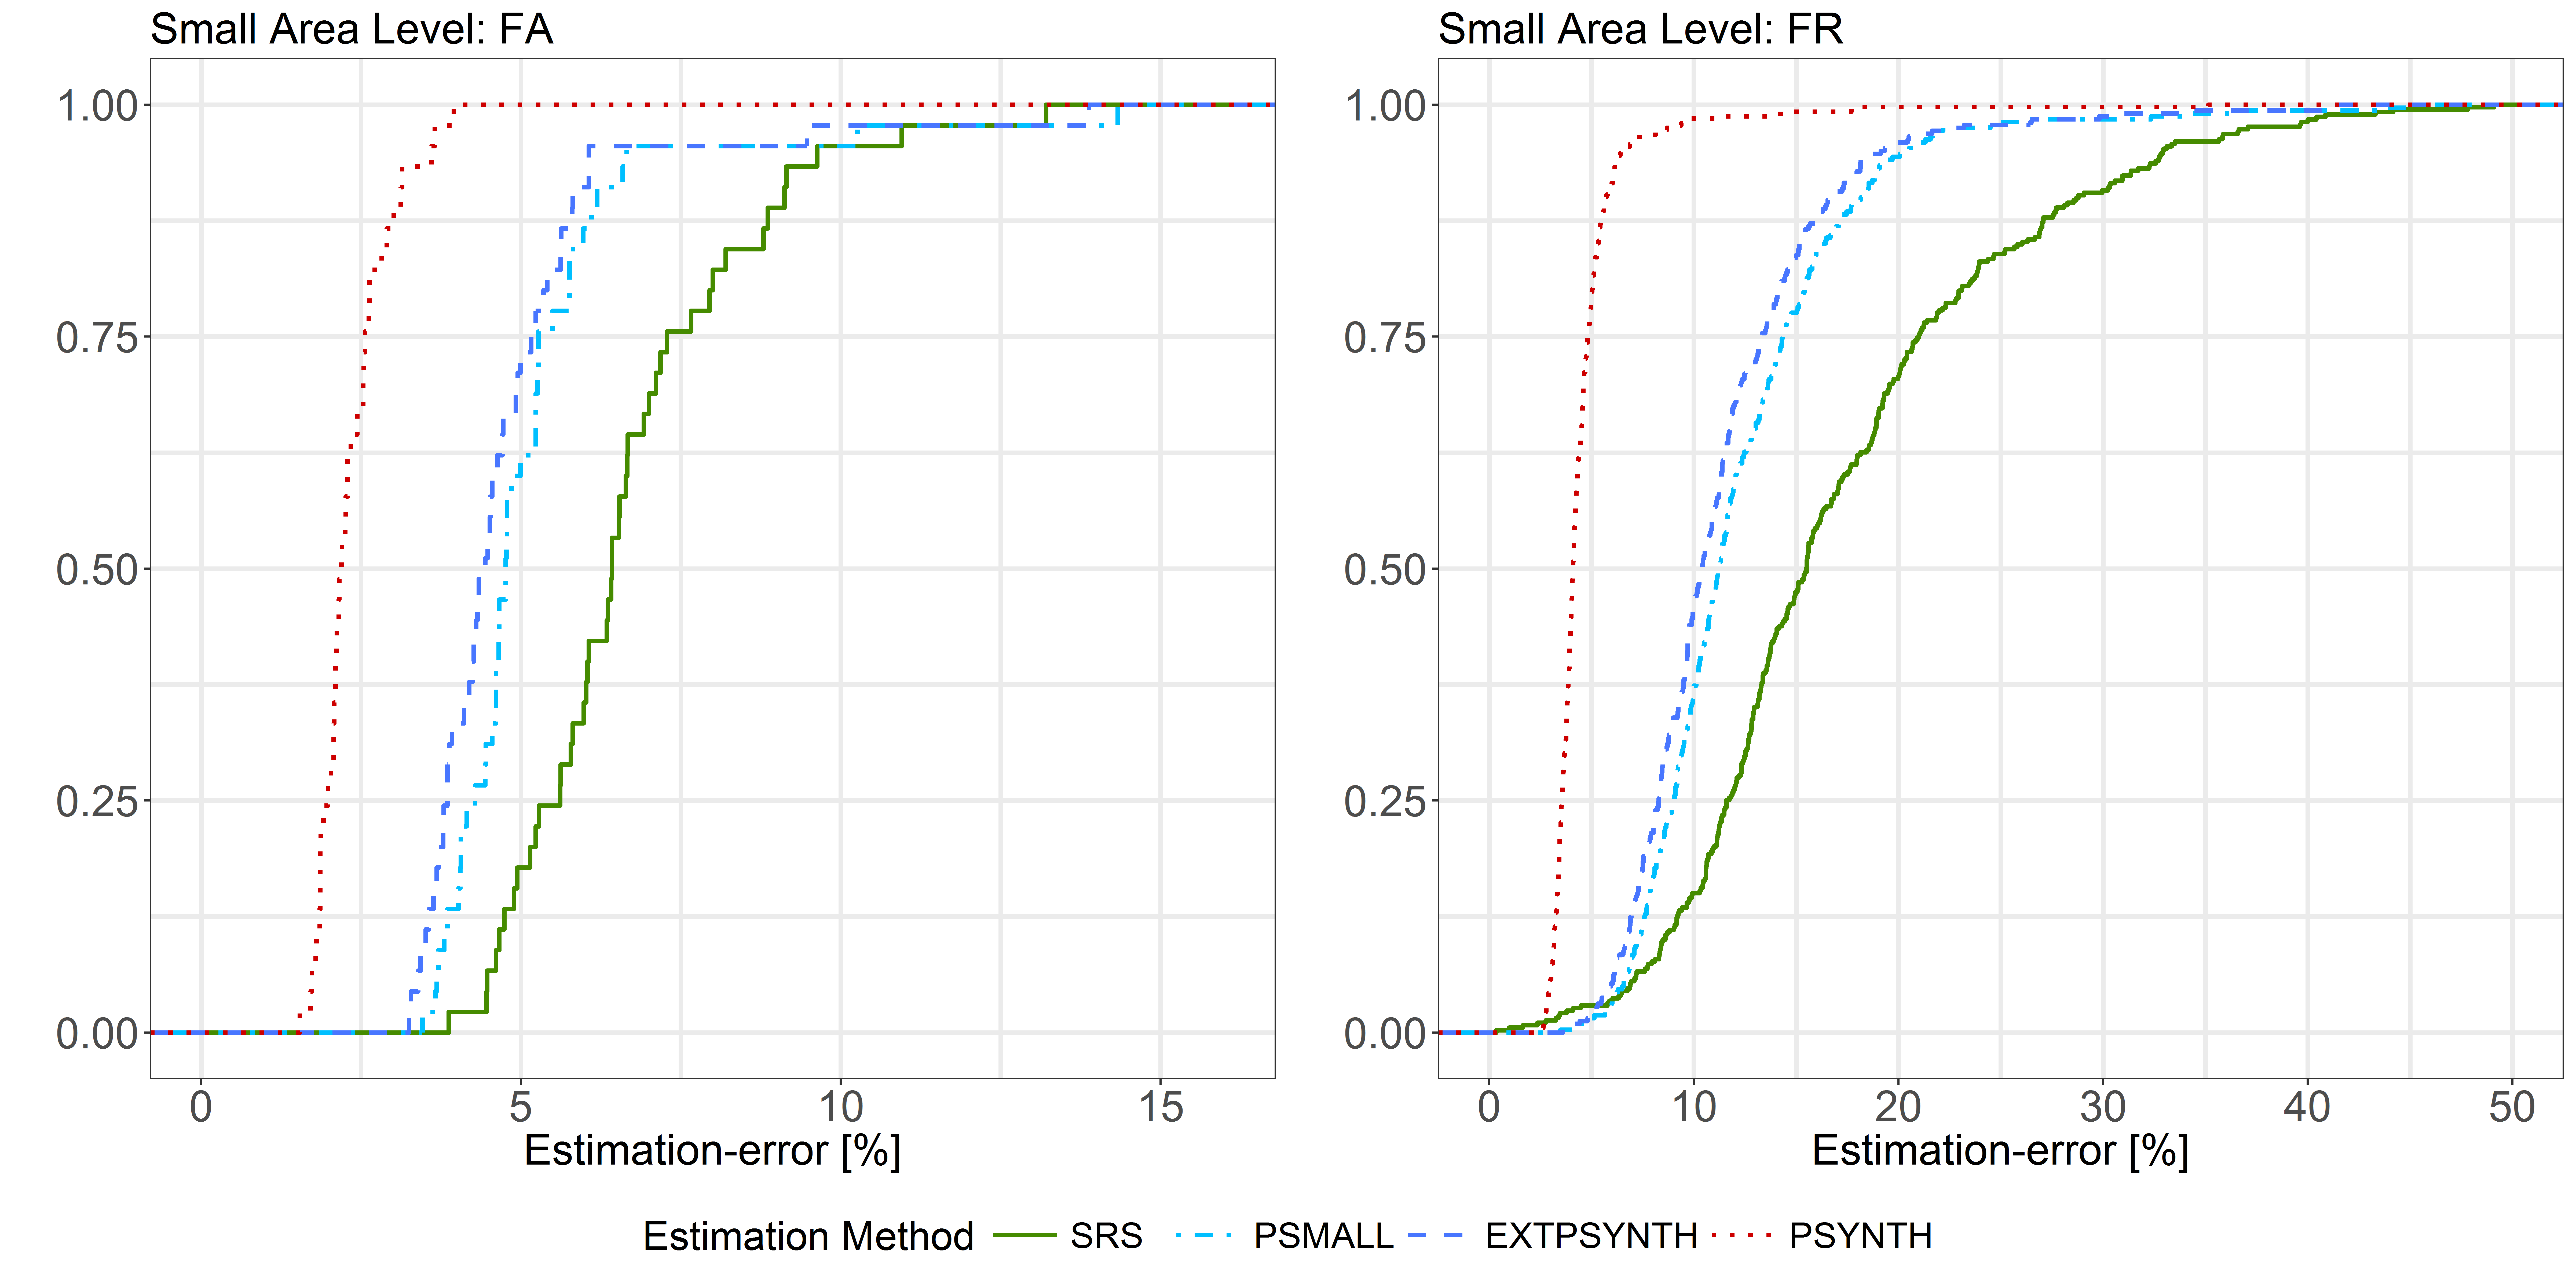
\includegraphics{fig/error_distr_foa_fu.png}}
	\caption{Cumulative distribution of estimation errors under SRS, \psmall{}, \extpsynth{} and the \psynth{} estimator. \textit{Left}: Results for the 45 FA units. \textit{Right}: Results for the 388 (SRS), 321 (\psmall{} / \extpsynth{}) and 403 (\psynth{}) FR units.}
	\label{fig:disterrors}
\end{figure}

On both small area levels, the \psynth{} estimator resulted in much smaller estimation errors compared to \psmall{} and \extpsynth{}. This was as expected, since the \psynth{} variance estimate does not take the residual variation in each small area unit into account (section \ref{sec:psynth}). Compared to the asymptotically design-unbiased estimators \psmall{} and \extpsynth{}, the estimation errors produced by \psynth{} thus seem to be too optimistic. One should also recall that the estimates of the \psynth{} estimator are potentially design-biased.

%% NOTES
 %Estimation errors smaller than 10\% were achieved for only 15\% (xx) of all FR units under SRS, while this proportion could be increased to 38\% and 46\% by PSMALL and EXTPSYNTH. 




% ----------------------------------------------------------------------- %
% ----------------------------------------------------------------------- %
\subsection{Comparison of \psmall{} and \extpsynth{}}
\label{sec:comp}

Figure \ref{fig:disterrors} reveals that the error distribution of \psmall{} and \extpsynth{} are very similar, with \psmall{} showing marginally higher estimation errors. In order to investigate the differences between \psmall{} and \extpsynth{}, we compared the g-weight variances of both estimators for all 321 FR units (fig. \ref{fig:compvar}, left). As obvious, \psmall{} yielded slightly larger variances for the vast majority of the estimates. As addressed in section \ref{sec:extpsynth}, one possible explanation for such differences was the effect of one or more cluster not entirely being included in a small area unit, as this would constitute a violation of the \extpsynth{} estimator. This violation was actually observed in 155 of the 321 FR units (48\%). 


However, the affected FR units (depicted in red diamonds, fig. \ref{fig:compvar}) did not show a significant divergence from the \psmall{} variances with respect to the remaining unaffected FR units. The variance differences between the two estimators were thus due to the mathematical formulations of the \psmall{} and \extpsynth{} estimator, which are asymptotically equivalent only under large terrestrial sample sizes $n_{2,G}$ within the small area \citep[pp.17--18]{mandallaz2016}. An additional comparison of the absolute differences in the g-weight variance (fig. \ref{fig:compvar}, right) revealed that large divergences did in fact particularly occur for small area units with small terrestrial sample sizes ($n_{2,G} \leq 5$). The differences decreased with increasing sample size and thus confirmed the asymptotic relationship between the two estimators. However, a comparison of the confidence intervals of \psmall{} and \extpsynth{} revealed that the variance differences did not lead to statistically significant point estimates.\par

% The results indicate that the adjustment of the intercept term to the data within a small area used in the \extpsynth{} estimator will in general yield slightly smaller variances than the \psmall{} estimator.

% NOTES:
% - Section \ref{sec:comp} provides a more detailed analysis of the differences between the two estimators.
% - DM-explanation: The model residuals and thus the residual variance for extpsynth should in general be a bit better than those of psmall, since we additionally adjust the regression
%                   to the small area data by introducing the sae-indicator variable (even if this is strictly speaken only a means to cause zero-mean-residuals)
%                   ==> we even can relate the differences to the residual variation, since the first and second term of extpsynth and psmall area identical with exception 
%                       of the adjusted regression coefficient
% - we can see the asymptotic of psmall and extpsynth: with increasing n2G, psmall and extpsynth are mathematically identical
% ==> so differences will particularly concern sae units with small n2G (threshold seems to be around n2G < 10)


\begin{figure}[H]
	\centering
	\resizebox{1\hsize}{!}{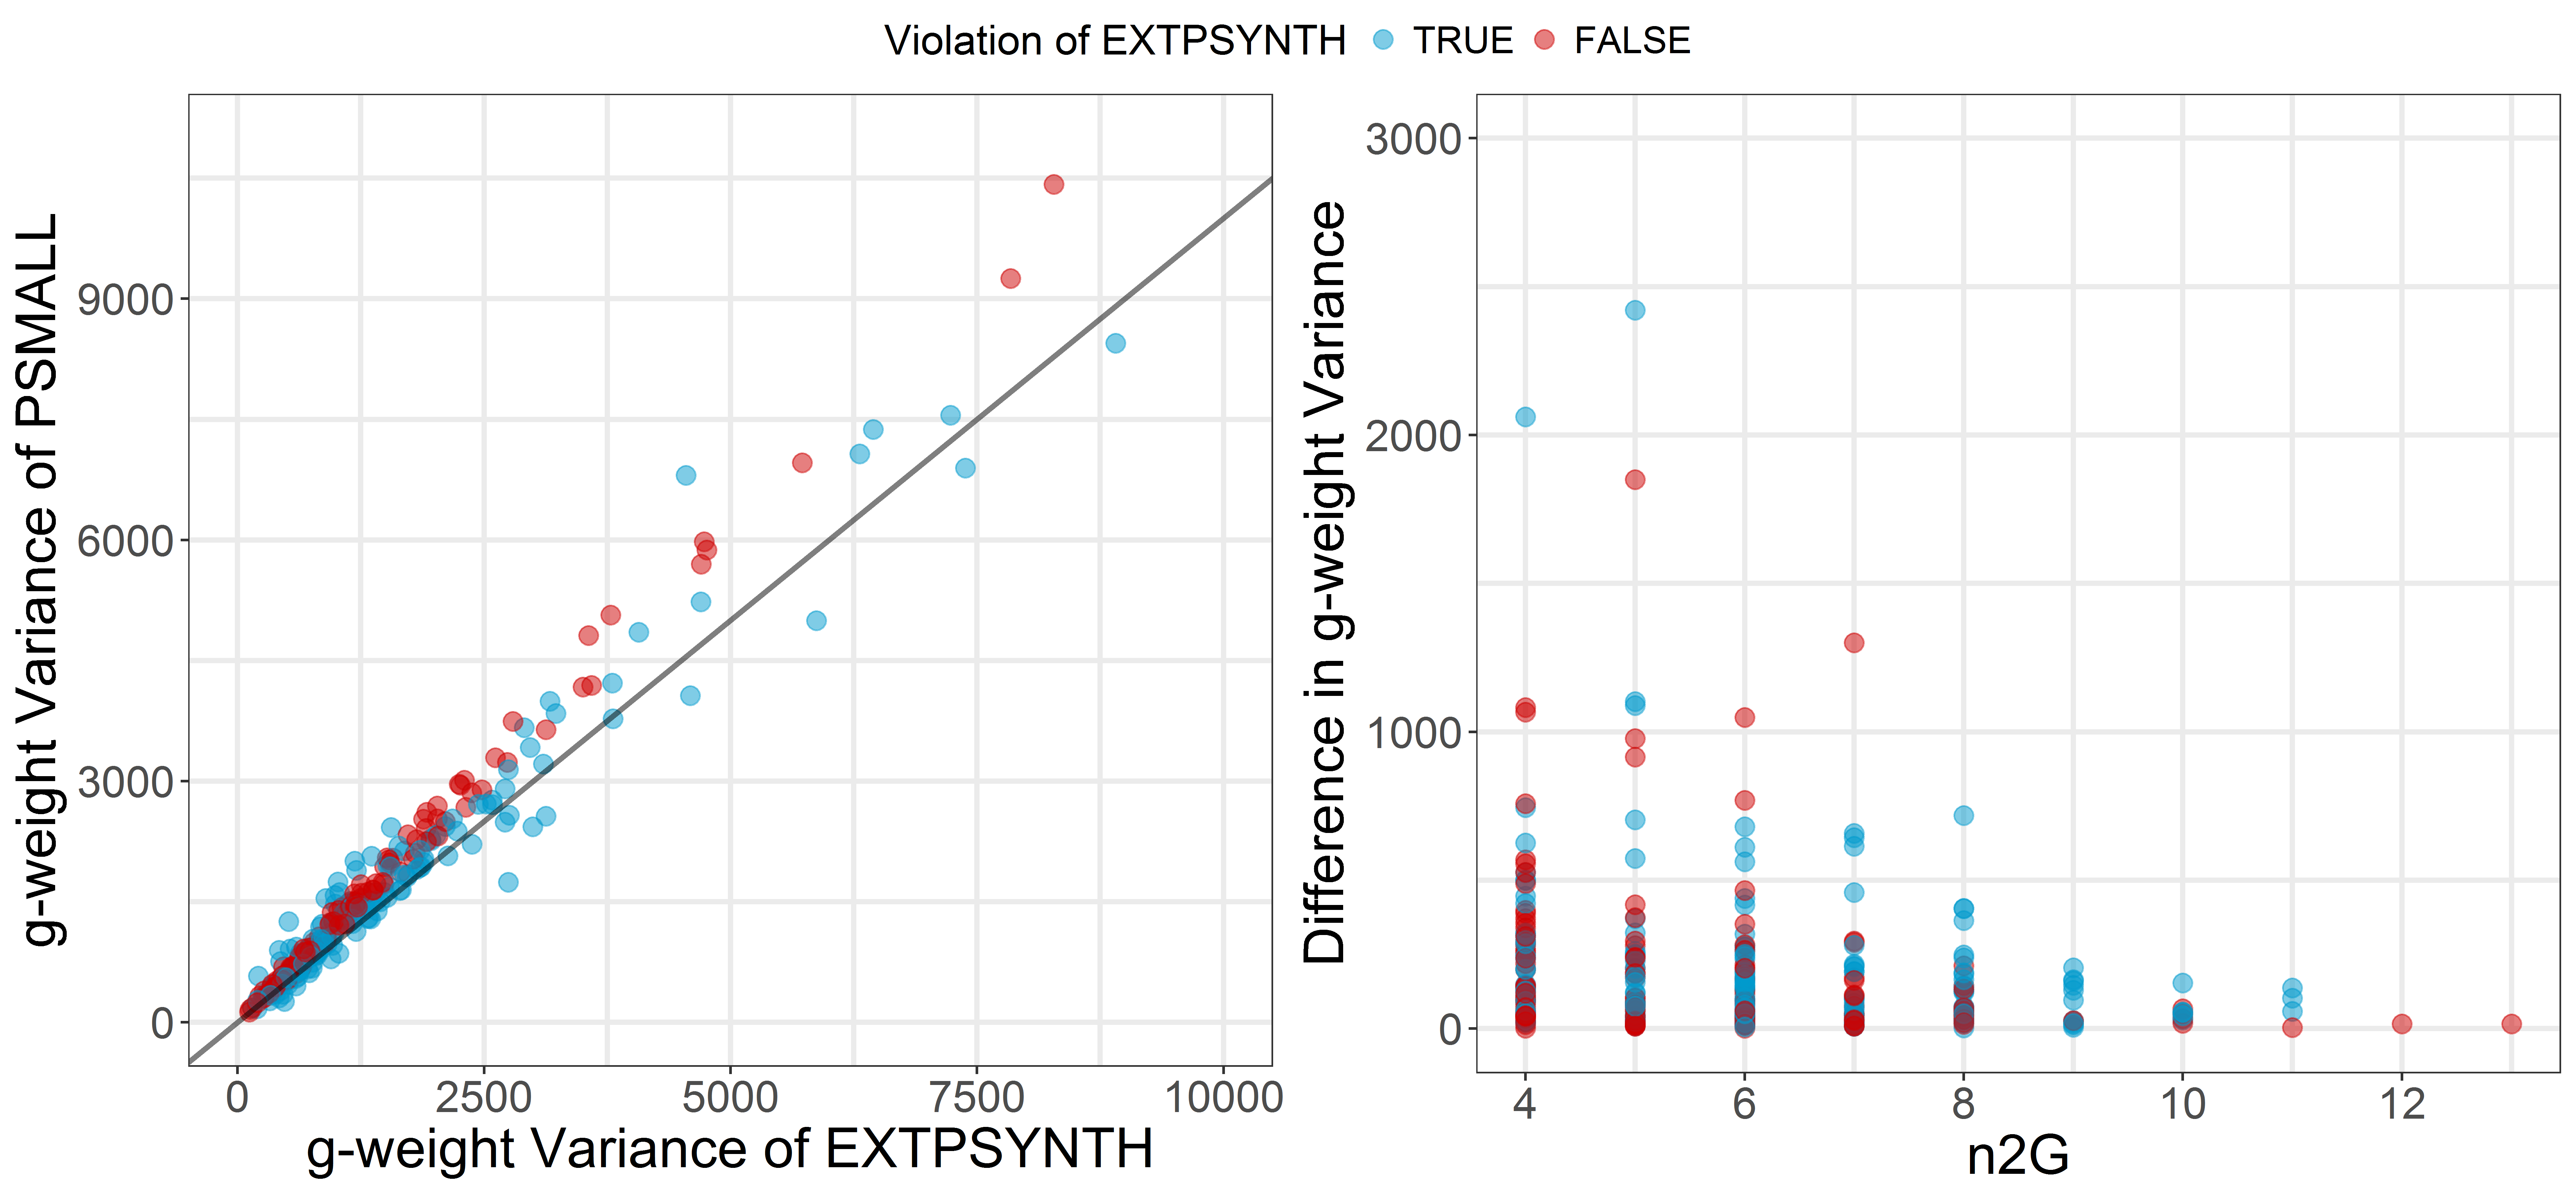
\includegraphics{fig/psmall_vs_extpsynth_fu.png}}
	\caption{\textit{Left}: Comparison of the g-weight variance between the PSMALL and the EXTPSYNTH estimator for the 321 FR units.
		\textit{Right}: Difference in g-weight variance between the PSMALL and the EXTPSYNTH estimator in dependence of the terrestrial data ($n2G$) in the FR unit.}
	\label{fig:compvar}
\end{figure}




% ----------------------------------------------------------------------- %
% ----------------------------------------------------------------------- %
\subsection{Variance reduction compared to SRS}
\label{sec:gain_eval}

The variance reduction relative to SRS for \psmall{} and \extpsynth{} are described in Figure \ref{fig:gain} and Table \ref{tab:gain}. A direct comparison of the variances within the small area units revealed that the application of the design-unbiased estimators (\psmall{}, \extpsynth{}) led to a variance reduction compared to SRS in all FA units. In 75\% of the FA units, the \extpsynth{} estimator was able to reduce the variance by up to 54.1\%. The reduction in variance can also be expressed in the relative efficiency values, which were 2.02 on average and ranged between 1.18 and 4.13 on the FA level. On FR level, the reduction in variance and the relative efficiencies reached even higher values (Table \ref{tab:gain} and Fig. \ref{fig:gain}). The \psmall{} estimator again yielded slightly lower variance reductions and relative efficiencies due to the generally smaller variances of the \extpsynth{} estimator (section \ref{sec:comp}).

\begin{figure}[H]
	\centering
	\resizebox{0.73\hsize}{!}{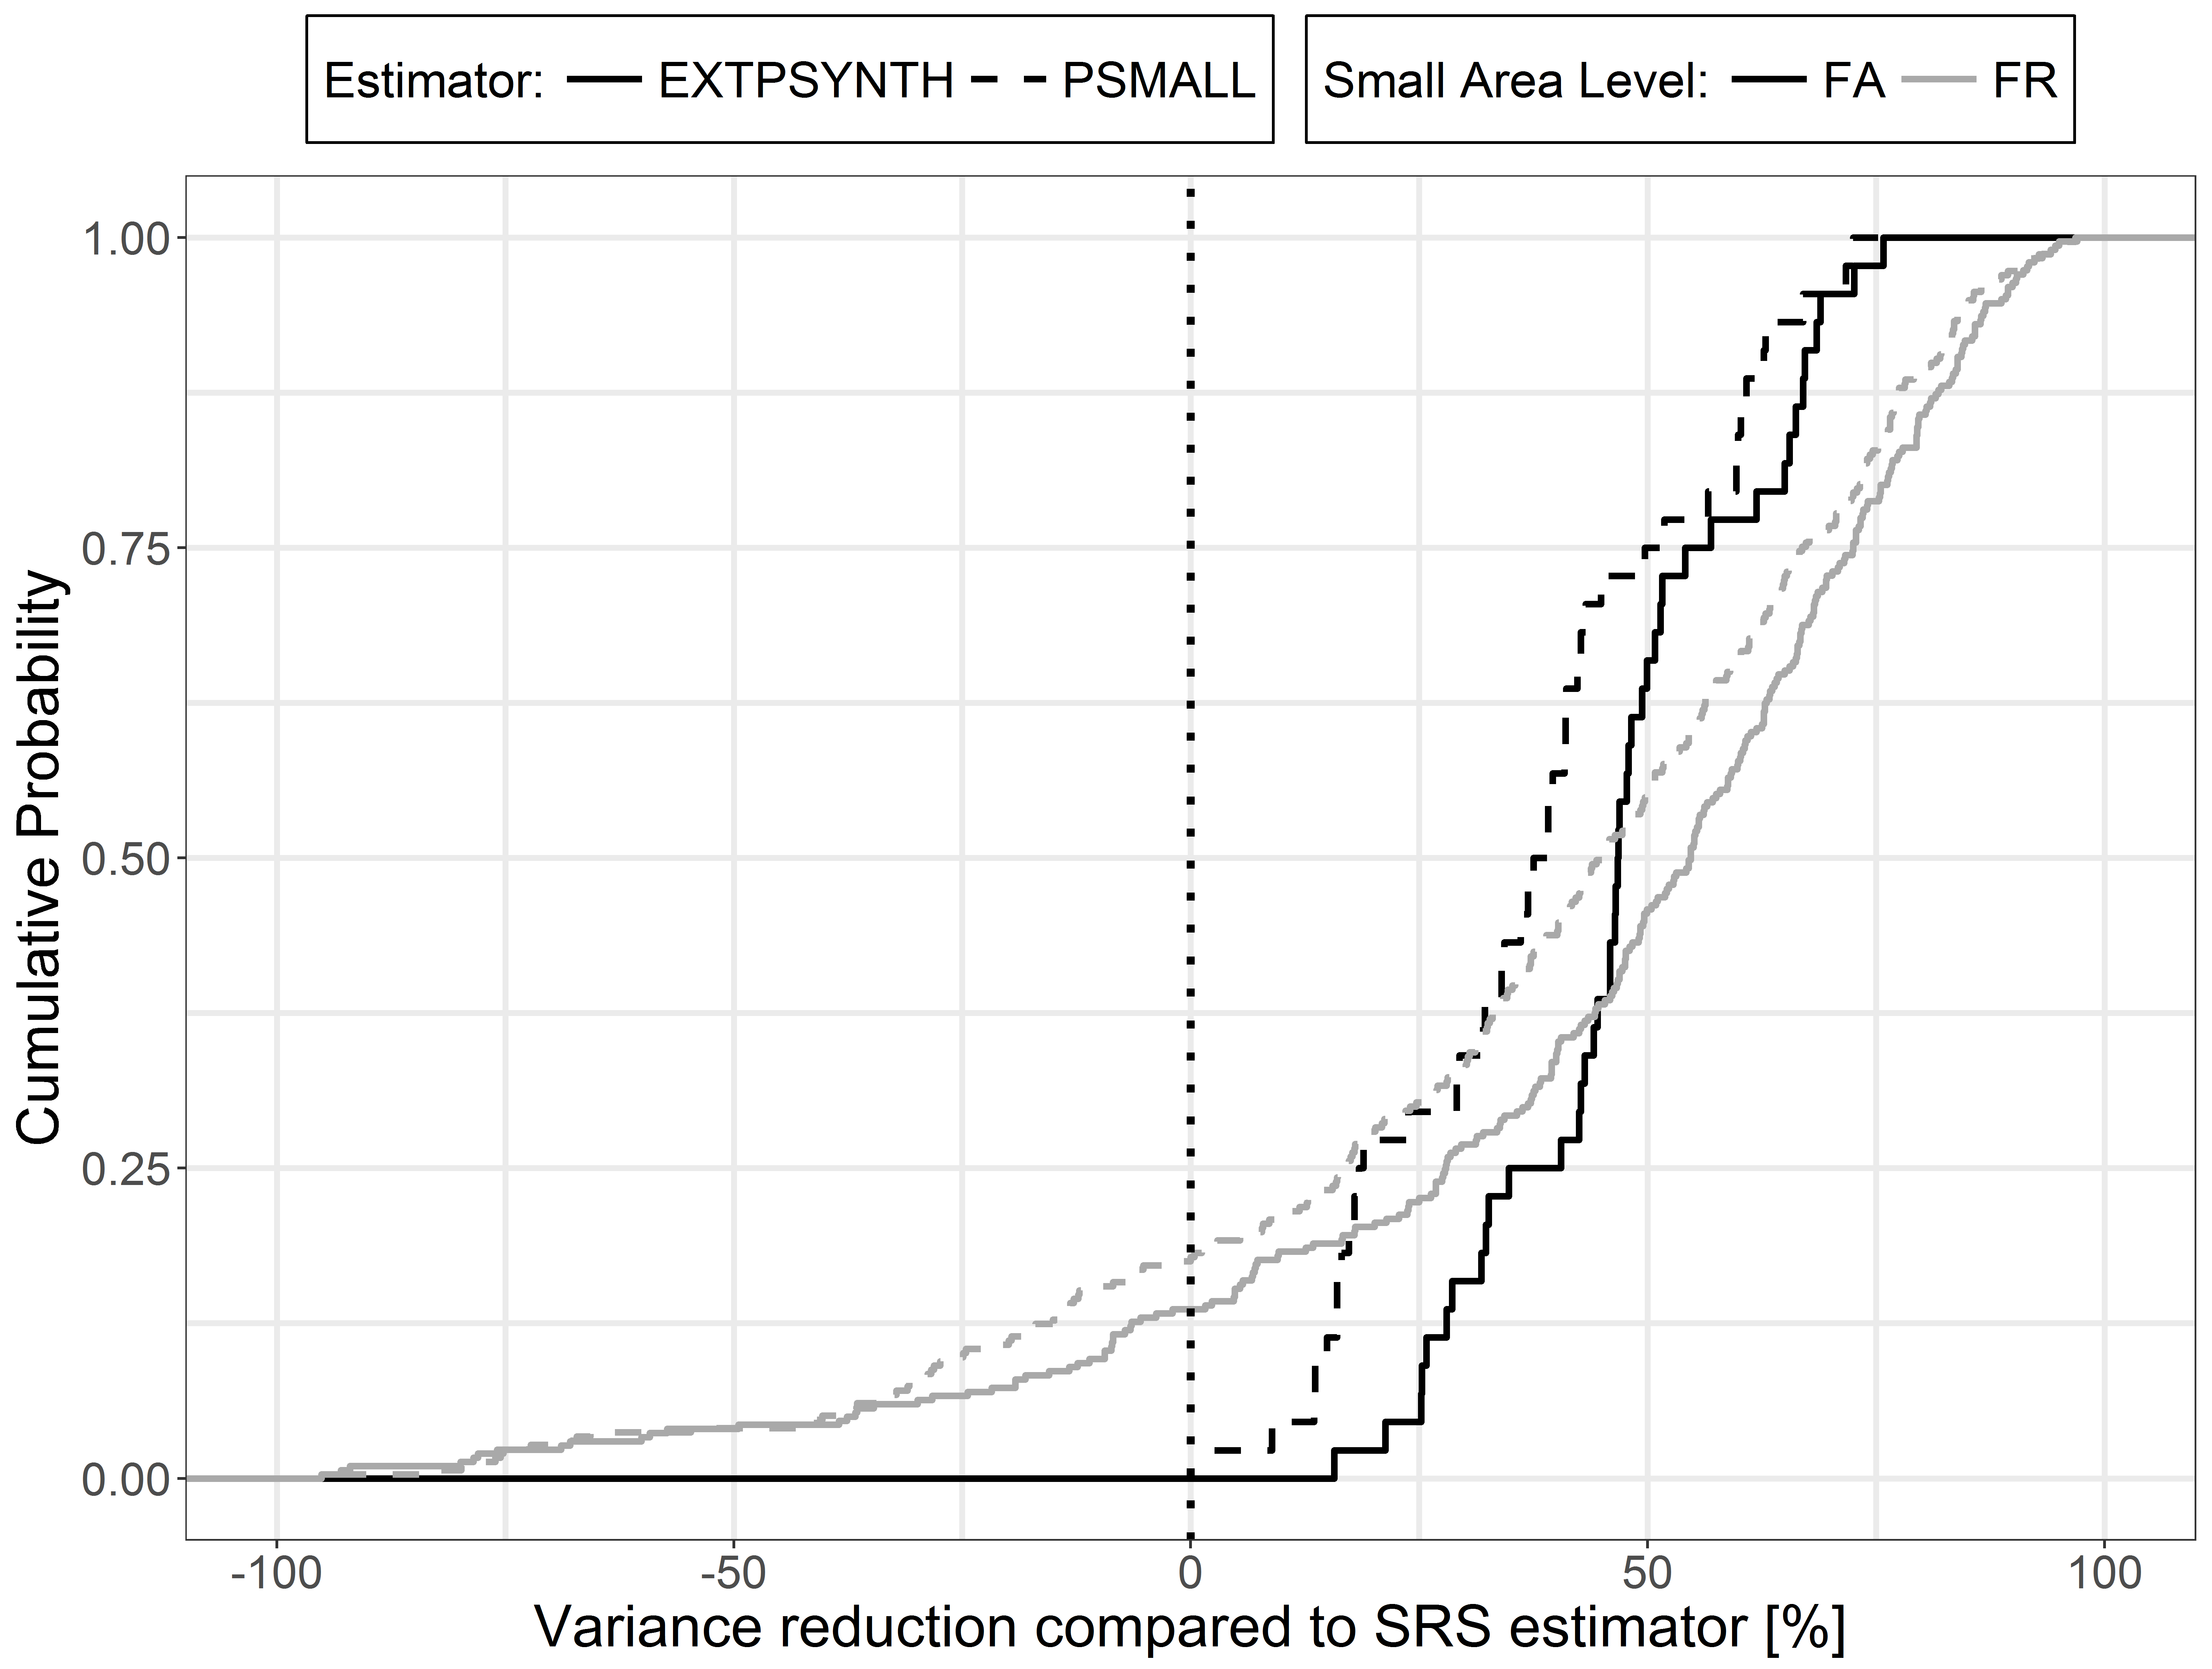
\includegraphics{fig/compare_onephase_extpsynth_psmall.png}}
	\caption{Cumulative distribution of variance reduction by the PSMALL and EXTPSYNTH compared to the SRS estimator for the  45 FA and 321 FR units.}
	\label{fig:gain}
\end{figure}

\begin{table}[H]
	\begin{center}
		\caption{Descriptive summary of variance reduction compared to SRS and relative efficiencies on the two forest district levels. $N_u$: number of evaluated small area units.}
		\vspace{0.2cm}
		\label{tab:gain}
		{\small %
			\begin{tabular}{c|l c|c c c|c c c} %8cols
				\hlineB{1}
				\multirow{2}{*}{District level} & \multicolumn{2}{c|}{\multirow{2}{*}{Estimator}} & \multicolumn{3}{c|}{Variance reduction [\%]} & \multicolumn{3}{c}{relative efficiency} \\
				\cline{4-9} & & & mean & min & max & mean & min & max \\
				\hline \hline
				\multirow{2}{*}{FA} & PSMALL    & ($N_u$=45)  & 33.51 &  2.6 & 72.5 & 1.74 & 1.03 & 3.64 \\
				& EXTPSYNTH & ($N_u$=45)  & 43.30 & 15.7 & 75.8 & 2.03  & 1.18 & 4.13 \\
				\hlineB{2}          
				\multirow{2}{*}{FR} & PSMALL    & ($N_u$=321) & 12.48 & -1203.9 & 96.8 & 2.54 & 0.08 & 31.61  \\
				& EXTPSYNTH & ($N_u$=321) & 24.75 & -892.7  & 97.0 & 2.95 & 0.10 & 33.70 \\
				\hline \hline
			\end{tabular}
		}%
	\end{center}
\end{table}

Cases also occurred on the FR level where one or both two-phase estimators produced larger variance values than under the SRS estimator. This happened in 19\% of the FR units under the \extpsynth{}, and in 24\% of the FR units under the \psmall{} estimator. One possible reason for this was supposed to be a large residual variance due to a poor performance of the regression model within the small area unit. In order to investigate this hypothesis, we analyzed the three variance terms of the \psmall{} estimator (eq. \ref{eq:psmallvar}), i.e. the variance introduced by the uncertainty of the regression coefficients (term 1), the variance caused by estimating the auxiliary means (term 2), and the variance of the model residual (term 3). In general, the residual term is expected to make the largest contribution to the overall variance since it's sample size is based on $n_{2,G}$ whereas the auxiliary term and the coefficient term are based on larger sample sizes, i.e. $n_{1,G}$ and $n_2$ respectively. Figure \ref{fig:fail} illustrates the share of the overall variance by the residual term of the \psmall{} estimator scaled by the overall percentage reduction or increase of the variance compared to SRS for various small area sample sizes $n_{2,G}$.\par

The residual term generally constitutes the dominating part of the \psmall{} variance (around 84\% on average). Although high residual term dominance does not necessary indicate that the \psmall{} variance will be disproportionately large, as apparent from Figure \ref{fig:fail} (\textit{right}), the vast majority of the small areas where the \psmall{} variance was larger than the SRS variance had residual terms contributing over 75\% to the overall \psmall{} variance. Furthermore, the magnitudes of the worst cases tended to occur in lower sample sizes. For example, of the FR units that saw variance increases where $n_{2,G}=4$, the average increase was 272\%, compared to 62\% for FR units with $n_{2,G} > 4$ (Fig. \ref{fig:fail}, \textit{left}).  In comparison, the magnitude of the variance decreases were far more homogeneous than for the variance increases regardless of terrestrial sample size. Since $n_{2,G}$ is the same for \psmall{} and SRS, this implies that the sum of square residuals for the model are likely larger than the sum of square local densities for the clusters in $s_{2,G}$ indicating the presence of outliers with large residuals in the problematic small areas. This situation is likely to arise when there was forest loss after the ALS scanning but before the terrestrial survey year. % [check that]

%As expected, the residual term generally constitutes the dominating part of the \psmall{} variance (around 84\% on average). However, a high proportion of the residual variance term seems not to be the driver for large \psmall{} variances, as apparent from Fig. \ref{fig:fail} (\textit{right}). The FR units where the \psmall{} estimator produced larger variances than the SRS estimator did not systematically differ from the majority of the FR units where \psmall{} performed better than SRS. However, FR units with exceptionally large variance increases compared to SRS particularly occurred under small terrestrial sample sizes of $n_{2,G} = 4$ (fig. \ref{fig:fail}, \textit{left}). These FR units exhibited a 272\% average increase of the SRS variance, compared to 62\% for the critical FR units with $n_{2,G} > 4$. In comparison, the achievable reduction in SRS variances compared to SRS were not considerably impacted by the terrestrial sample size (fig. \ref{fig:fail}, \textit{right}). The average reduction of these units was around 50\% under sampling sizes of both $n_{2,G} = 4$ and $n_{2,G} > 4$. 

\begin{figure}[H]
	\centering
	\resizebox{1\hsize}{!}{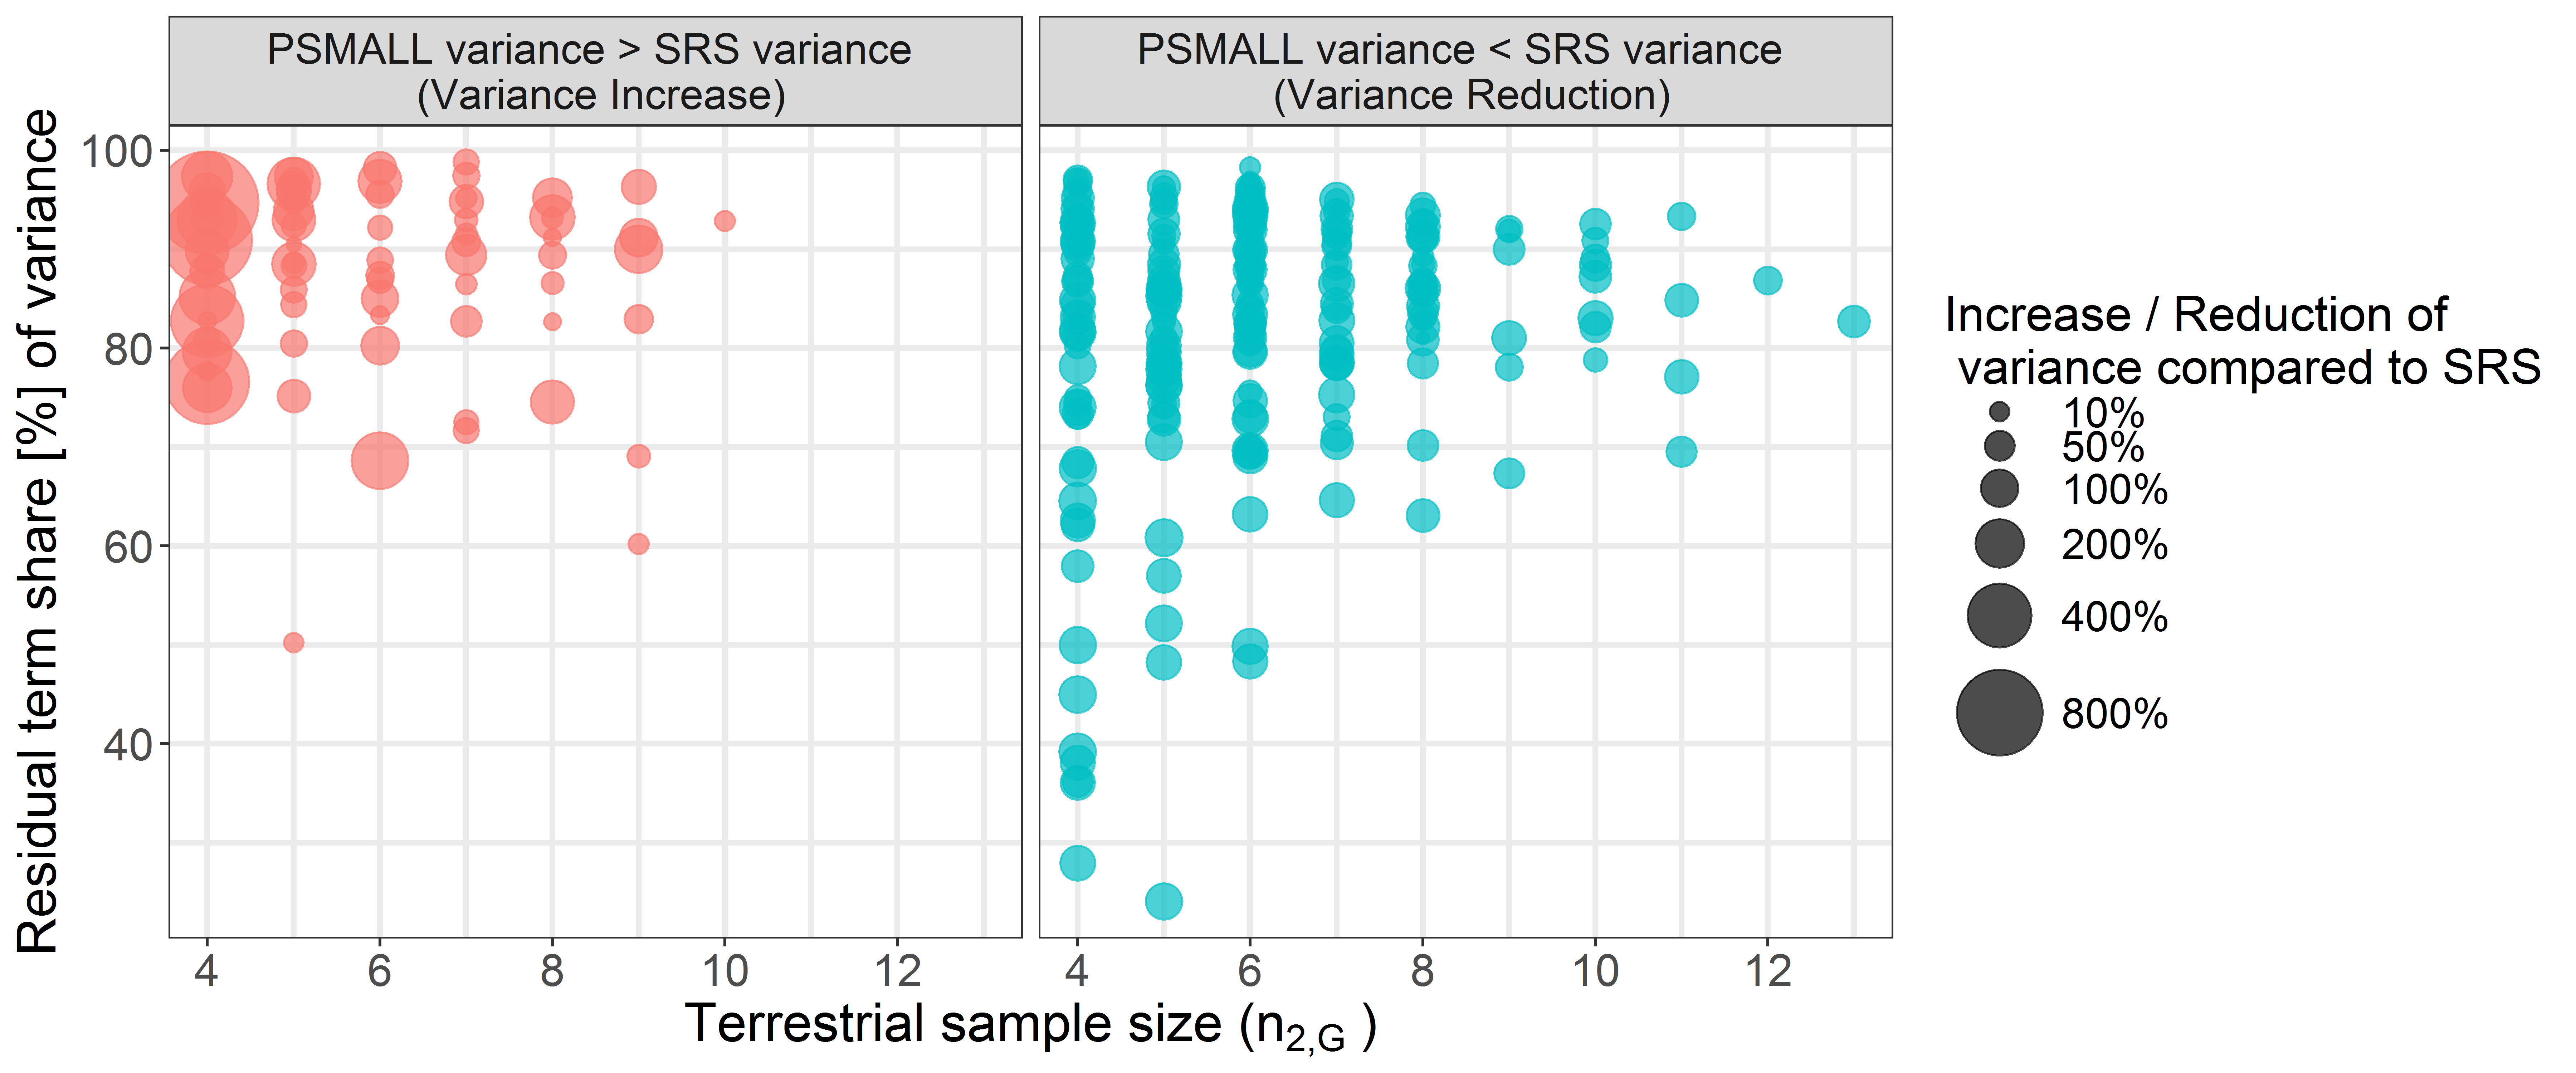
\includegraphics{fig/eval_2phase_fail_11.png}}
	\caption{Increase or reduction of the SRS variance by application of the \psmall{} estimator for all 321 FR units in dependence of a) the terrestrial sample size in the FR units (\textit{x-axis}) and b) the residual term proportion of the \psmall{} g-weight variance (\textit{y-axis}).}
	\label{fig:fail}
\end{figure}




% discussion: This also underlined why the \psynth{} estimator, which does not take the residual variation into account, produced substantially smaller variances than the design-unbiased estimator. 
% These findings suggest that moderate or poor model fits within a small area can cause the \psmall{} and \extpsynth{} estimator to produce higher variances than the SRS estimator particularly under small terrestrial sample sizes.



%\begin{figure}[H]
%	\centering
%	\resizebox{1\hsize}{!}{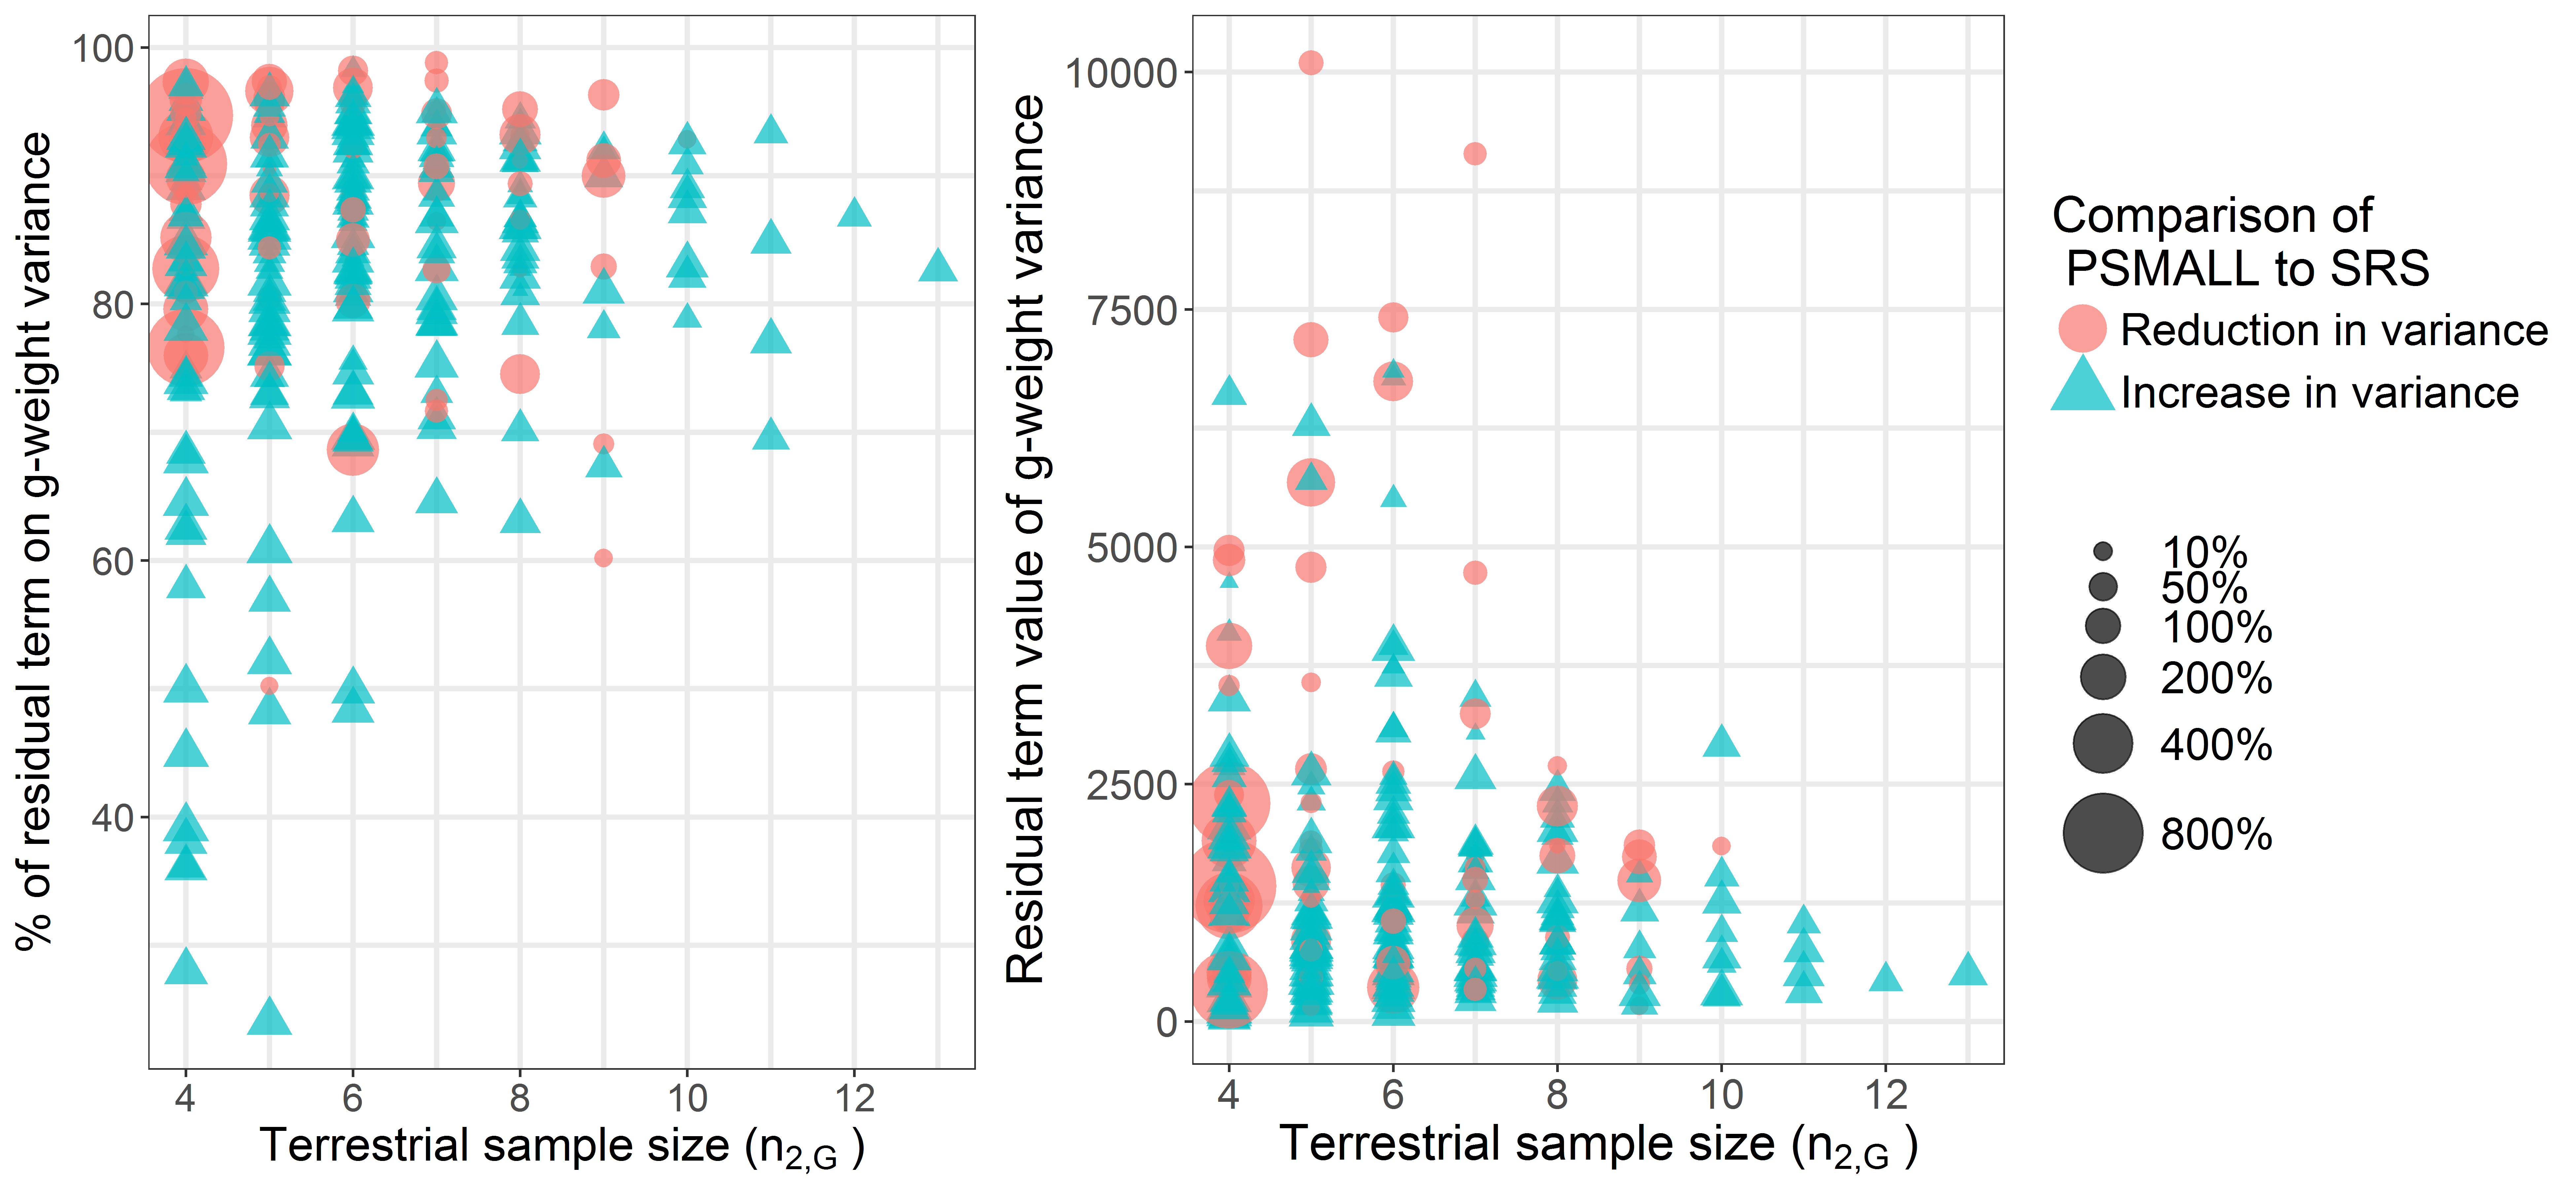
\includegraphics{fig/eval_2phase_fail.png}}
%	\caption{}
%	\label{fig:fail1}
%\end{figure}


% However, small terrestrial sample sizes can also have the effect that the SRS estimator might not reflect the actual variation of the local density within a small area. In this case, the two-phase variance estimate might be larger but more realistic. Whereas a visual analysis of aerial images, remote sensing data or stand maps might give some evidence for this hypothesis, a definite proof is practically infeasible.

\newpage\cleardoublepage


%============================================ Discussion ==========================================================%

\section{Discussion} %article
\label{sec:Dis}

% ----------------------------------------------------------------------- %
% ----------------------------------------------------------------------- %
%\subsection{Stratification according to ALS Acquisition Years and Tree Species}
%\label{sec:strat_dis}


% NOTES:
%
% - extension to change estimation
%   o BDOM more frequently updated, max. 1 year time gap between CHM and BWI3 survey
%   o also treespecies classific. frequently updated using sentinel 2 data
%   o the gain in model accuracy will certainly considerably increase if the ALSyear stratification becomes unnecessary Value increase also in combination with
%     further explanatory variables such as growing conditions
%
% - transfer of the suggested procedure to FDI inventories: maybe possible to get qunatified data for stands with acceptable estimation errors? (would be of high interest)
%
% - main findings:
%   o FA-level: 
%     + problem of large estiamtion errors solved on FA-level (average error of 5\%, 95\% <= 6.6%)
%
%   o FR-level:
%     + in most FR units (95\%), errors could be limited to 20\% compared to 40\% under SRS (status quo)
%     + however, the FA error level could not be achieved, due to much smaller sample sizes on the FR level
%     + 
%
%
% - the extpsynth estimator seems to generally produce slightly smaller variances and est. errors than psmall. This most probably caused marginally smaller residuals in the small area unit due to the adjustment of the intercept (which is primarily a means to ensure the zero-mean-residual property). Our analysis indicated that the difference between the two estimators get negligible for sample sizes > 10 due to their asymptotic relationship. Reassuringly, violations of the extpsynth estimator by one or more clusters not entirely included in G did not have an impact on the estimates.
%
% - our advice: if possible, calculate both estimators (two opinions). Differences might reveal undetected patterns in the data.
%
% - the decision wether the errors are acceptable cannot be answered here but (in our opinion) depend on the question whether ... decisions can be made based on the provided Confidence Intervals.
% - in a next step, we will investigate whether the derived confidence intervals are sufficient to be used as a validation for the stand-wise inventories (Kuliesis et al.)
% 
%
%
%
%
%
%
%
% - Kuliesis et al.:  --> "NFI [provide reliable estimates for the most important attributes and] can be used 
%                          as a tool for validation of all other inventories", i.e. stand-wise inventories
%                     ==> in our case, we can say that we illustrated how the German NFI data can now be used
%                         for this purpose, i.e. providing of reliable data to validate the stand-wise inventories
%














\newpage\cleardoublepage

%==================================== Conclusion & Outlook ==========================================================%

%\section{Conclusion}
\label{sec:concl}

The study led to two major conclusions: (1) the \extpsynth{} and \psmall{} estimator generally achieved substantially smaller estimation errors on the two investigated forest district levels compared to the SRS estimator. The demonstrated double-sampling procedure thus constitutes a major contribution to an increase in value of the existing German NFI data on the federal state level. However, it is not possible to conclude from our study results alone whether the realized error levels are already acceptable in order to support forest planning decisions. Thus, further investigations are necessary in close cooperation with the forest authorities. A first study will concentrate on testing the \extpsynth{} and \psmall{} confidence intervals as a validation source for the stand-wise inventories. (2) Despite the quality restrictions in the ALS data and the tree species map, the two data sources were found to be well suited to model the mean timber volume on plot and cluster level. With respect to frequently updated aerial canopy height models and tree species maps, it will thus be of hight interest to investigate the model and estimation accuracies that can be expected for future applications. In this framework, the incorporation of additional auxiliary data and the extension to change estimation seem the reasonable next steps to be explored towards an operational implementation of the demonstrated double-sampling procedure.\newpage\cleardoublepage


%============================================ Acknowledgements ==========================================================%


\section*{Acknowledgements}
\thispagestyle{plain}
We want to express our gratitude to Prof. H. Heinimann (Chair of Land Use Engineering, ETH Zurich) for supporting this study. We also want to explicitly thank Johannes Stoffels and Henning Buddenbaum from the Environmental Sensing and Geoinformatic Group of University of Trier for providing the ALS data and tree species classification map, and Kai Husmann and Christoph Fischer from the Northwest German Forest Research Institution Göttingen for their advice in processing the terrestrial inventory data. Special gratitude is also owed to Thomas Riedel from the Th{\"u}nen Institute for supporting this study and providing the densified NFI sample grid and Alexander Massey for proofreading.
\newpage\cleardoublepage


%============================================ Appendices ==========================================================%

%\appendix
\section{Appendix}
\label{sec:appendix_saerlp}

% -------------------------------------- %
\subsection*{R-squared on cluster level}

The R$^2$ on the cluster level is calculated using the number of plots $M(x)$ of each cluster in order to weight for the varying number of plots on which $Y_c(x)$ and $\hat{Y}_{c}(x)$ are based on. 

\begin{equation*}\label{eq:R_squared_clust}
R^2 =  \frac{\sum_{x \in s_2} \Big(\frac{M(x)}{\bar{M_2}}\Big)^2 \Big(\hat{Y}_{c}(x)-\hat{\bar{Y}}_c\Big)^2}{\sum_{x \in s_2} \Big(\frac{M(x)}{\bar{M_2}}\Big)^2 \Big(Y_{c}(x)-\hat{\bar{Y}}_c\Big)^2}
\end{equation*}

\noindent $Y_c(x)$ and $\hat{Y}_{c}(x)$ are the predicted and observed local densities on the cluster level calculated according to equations \ref{eq:locdens_clust} and \ref{eq:globresids}. $\hat{\bar{Y}}_c$ is the estimated sample mean corresponding to the weighted mean over all observed local densities on the cluster level (equ. \ref{eq:srs_est_clusters}).\par

% -------------------------------------- %
\subsection*{RMSE on cluster level}

The same weights $M(x)$ are also applied to calculate the RMSE on the cluster level. $n_2$ is the number of clusters used in the modeling frame.

\begin{equation*}\label{eq:RMSE_clust}
RMSE= \sqrt{\frac{1}{n_{2}}  \sum_{x \in s_2} \Big(\frac{M(x)}{\bar{M}_2}\Big)^2 \Big(\hat{Y}_{c}(x)-Y_c(x)\Big)^2}
\end{equation*}

\noindent The \textit{relative} or \textit{normalized} RMSE is calculated by setting the absolute RMSE in relation to the estimated sample mean $\hat{\bar{Y}}_c$:

\begin{equation*}\label{eq:NRMSE_clust}
RMSE[\%] = \frac{RMSE}{\hat{\bar{Y}}_c}
\end{equation*}

\noindent Generally note that the weights $\frac{M(x)}{\bar{M_2}} \equiv 1$ if the number of plots per cluster is constant.
\newpage\cleardoublepage


%============================================ Literature ==========================================================%

\bibliography{bib/literaturerRLPsae}\newpage\cleardoublepage
    

%==================================================================================================================%
\end{document}













